\chapter{പെണ്ണരശുനാടോ? കേരളമോ?}
\label{chapter2}  

\begin{figure}[h]
\begin{center}
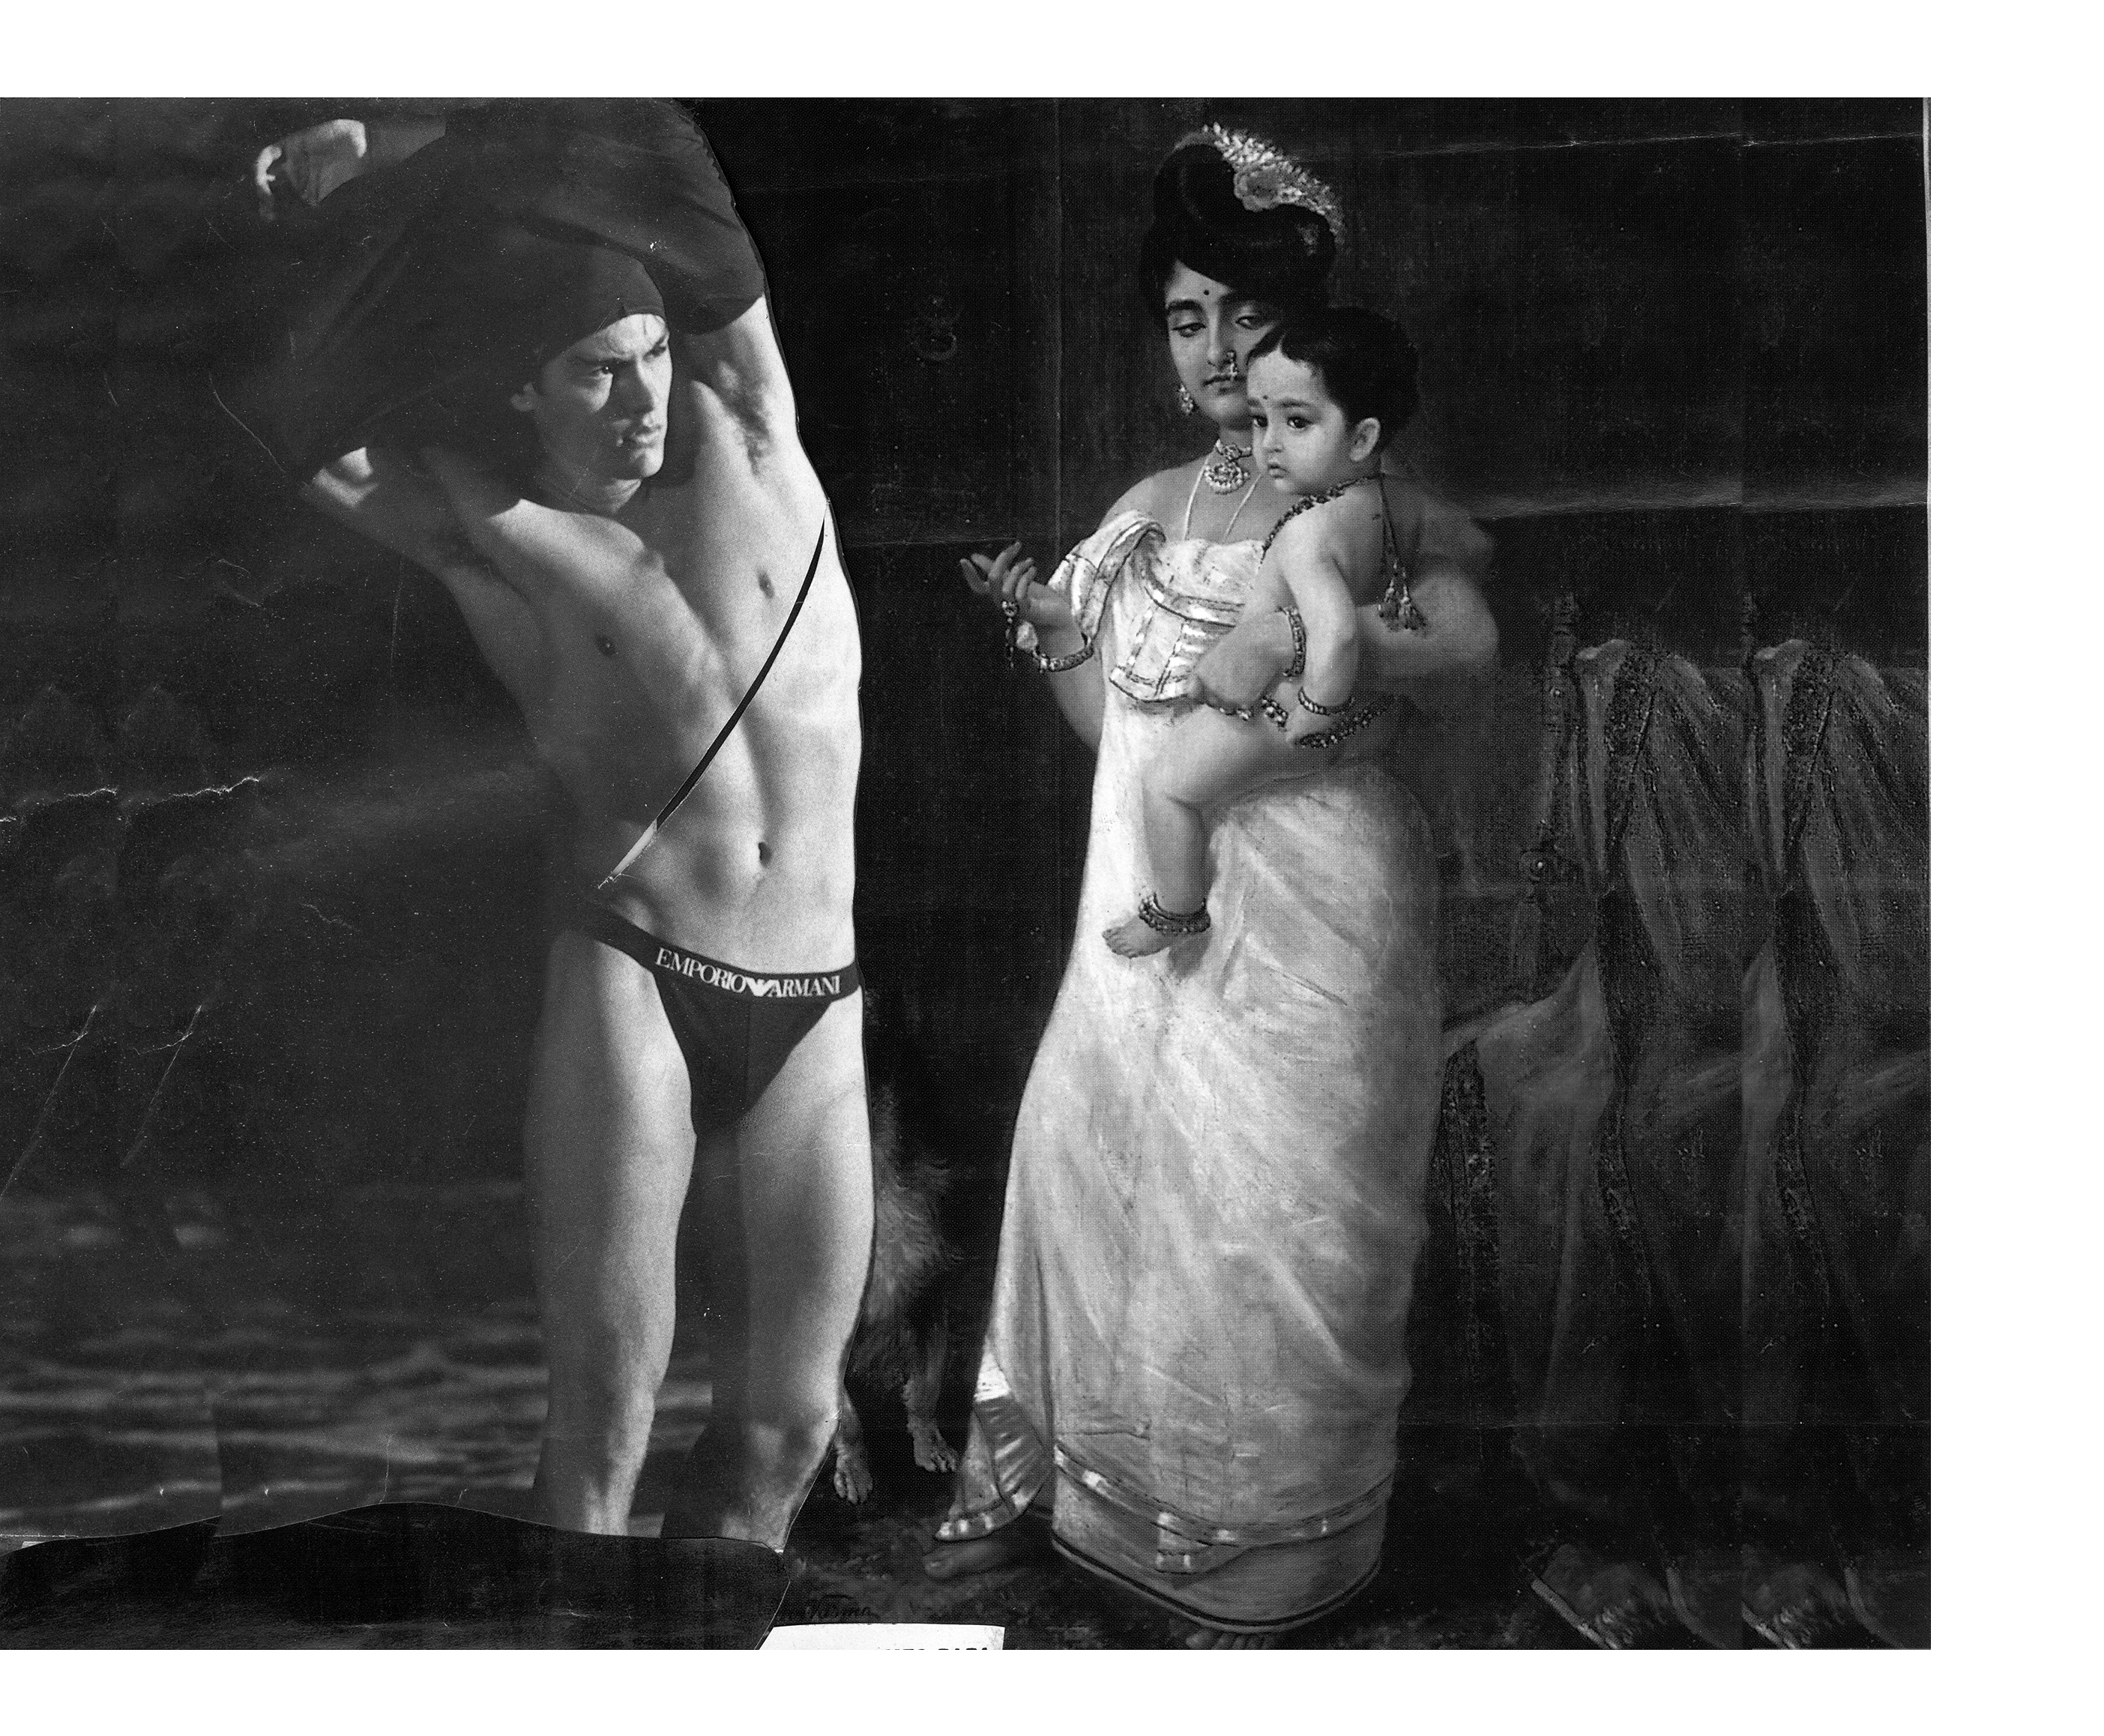
\includegraphics[width=\textwidth,height=10cm]{Kulasthree_Chapter02_pic01.jpg}
\end{center}
\end{figure}

\textit{\paragraph{}
 മരുമക്കത്തായികളായിരുന്ന മലയാളികൾക്കിടയിൽ സ്ത്രീകൾ വളരെ സ്വതന്ത്രരായിരുന്നുവെന്ന അവകാശവാദം നാം സാധാരണ കേൾക്കാറുള്ളതാണ്. വിവാഹം, സ്വത്തവകാശം എന്നീ രണ്ടുകാര്യങ്ങളിൽ മരുമക്കത്തായം പിന്തുടർന്നിരുന്ന സമുദായങ്ങളിലെ സ്ത്രീകൾക്ക് ആനുകൂല്യമുണ്ടായിരുന്നുവെന്ന് നമുക്കറിയാം. എന്നാൽ ഇതുകൊണ്ടുമാത്രം കേരളം 'പെണ്ണരശുനാടാ'യിരുന്നുവെന്ന് പറയാനൊക്കുമോ? ദൈനംദിനജീവിതത്തിന്റെ ഭാരം മേലാളസ്ത്രീകൾക്ക് കുറവായിരുന്നോ? മാത്രമല്ല, വരേണ്യസ്ത്രീകളുടെ അനുഭവത്തെമാത്രം കണക്കാക്കുന്ന രീതി തീർച്ചയായും ചരിത്രരചനയിൽ ആശാസ്യമല്ല. കീഴാളസ്ത്രീകളുടെ അനുഭവങ്ങൾകൂടി കണക്കാക്കിയാൽ 'സ്ത്രീസ്വാതന്ത്ര്യ'ത്തെ പരമ്പരാഗതമായി പോഷിപ്പിച്ച സമൂഹം' എന്ന പേരിന് നാം അർഹരല്ലെന്നു കാണാം.}
 
 \section{'ജന്മഭേദവ്യവസ്ഥ'യിലെ സ്ത്രീകൾ}


\paragraph{}'സ്ത്രീകൾ ഭരിക്കുന്ന നാട്' എന്ന് ഇന്ന് കേരളത്തെ ആരെങ്കിലും വിശേഷിപ്പിച്ചാൽ ആ വ്യക്തിക്ക് തീരെ അറിവില്ലെന്നേ നാം വിചാരിക്കൂ. പക്ഷേ പണ്ട്, അതായത് പത്തൊമ്പതാം നൂറ്റാണ്ടിൽ, കേരളത്തിന് 'പെണ്ണരശുനാട്' അഥവാ 'പെൺഭരണം നിലവിലുള്ള നാട്' എന്നു പേരുണ്ടായിരുന്നു. മരുമക്കത്തായ കുടുംബരീതികൾ സ്ത്രീകൾക്കനുവദിച്ചിരുന്ന ചില തെരഞ്ഞെടുപ്പുകളെക്കുറിച്ചായിരിക്കാം ഇതു സൂചിപ്പിക്കുന്നത്. മരുമക്കത്തായ കുടുംബവ്യവസ്ഥയിൽ ചില ഘടകങ്ങൾ സ്ത്രീകൾക്കനുകൂലമായിരുന്നുവെന്ന വസ്തുത ഇന്ന് പരക്കെ അംഗീകരിക്കപ്പെടുന്നുണ്ട്. എന്നുവച്ച് മരുമക്കത്തായികളായ സ്ത്രീകൾ 'സർവ്വസ്വതന്ത്രകൾ' ആയിരുന്നില്ലെന്നു നമുക്കറിയാം. മരുമക്കത്തായത്തിൽ - അതായത് സ്വത്തവകാശം ഒരു തലമുറയിൽനിന്ന് അടുത്തതലമുറയിലേക്ക് നീങ്ങുന്നത് പെൺവഴിക്കായിരുന്ന രീതിയിൽ - സ്ത്രീകൾക്ക് കൂടുതൽ നിലയും വിലയുമുണ്ടായത് സ്വാഭാവികംമാത്രം. കാരണം, കുടുംബം തുടരുന്നത് പെണ്മക്കളുടെ മക്കളിലൂടെയാകുമ്പോൾ മകൾക്ക് ഒരുവിധം നല്ല പരിഗണന കൊടുത്തല്ലേ പറ്റൂ?

\paragraph{}മലയാളികൾ എല്ലാവരും മരുമക്കത്തായികളായിരുന്നില്ലെന്ന് ഓർക്കേണ്ടതുണ്ട്. കുടുംബത്തിന്റെ പിന്തുടർച്ച ആൺമക്കളിലൂടെ കണക്കാക്കിയിരുന്ന മക്കത്തായവ്യവസ്ഥ പിന്തുടർന്നവരും (ഉദാഹരണത്തിന്, സുറിയാനി ക്രിസ്ത്യാനികൾ, നമ്പൂതിരിമാർ) മക്കത്തായ-മരുമക്കത്തായവ്യവസ്ഥകളെ കൂട്ടിയിണക്കി 'മിശ്രദായം' അംഗീകരിച്ചിരുന്നവരും (ഉദാഹരണത്തിന് ഈഴവരിൽ ചില വിഭാഗക്കാർ) ഇവിടെയുണ്ടായിരുന്നു. ഇക്കൂട്ടർക്കിടയിൽ സ്ത്രീകൾക്ക് ഔപചാരികനിലയിൽ ഒരുപാട് അധികാരമുണ്ടായിരുന്നുവെന്ന് പറയാൻ കഴിയില്ല. അതുകൊണ്ട് കേരളത്തെ ഒന്നടങ്കം 'പെണ്ണരശുനാടെ'ന്ന് വിശേഷിപ്പിച്ചത് ശരിതന്നെയോ എന്ന ചോദ്യം പ്രസക്തമാണ്. കേരളത്തിലെ എല്ലാ സ്ത്രീകൾക്കും ഒരുപോലെ ബാധകമായ ഒരു സ്ത്രീസങ്കല്പം, അല്ലെങ്കിൽ സ്ത്രീത്വാദർശം, പരമ്പരാഗത മലയാളിസമൂഹത്തിൽ ഉണ്ടായിരുന്നില്ലെന്നു പറയാം. പരമ്പരാഗത കേരളീയ സമൂഹത്തെ 'ജന്മഭേദവ്യവസ്ഥ' എന്നു നമുക്കു വിളിക്കാം. ഒരു വ്യക്തി ഏതു ജാതിവിഭാഗത്തിൽ ജനിക്കുന്നുവോ, ആ വിഭാഗത്തിന്റെ പൊതുനിയമങ്ങൾക്ക് അടിപ്പെട്ട് ജീവിതകാലം മുഴുവൻ കഴിച്ചുകൂട്ടിക്കൊള്ളണമെന്ന നിബന്ധന ഇതിന്റെ അടിസ്ഥാനപ്രമാണങ്ങളിലൊന്നായിരുന്നു.


\paragraph{}ഒരു ജാതിയിൽ ജനിച്ചാൽ മറ്റൊരു ജാതിയിലേക്കു മാറാൻ മിക്കപ്പോഴും കഴിയില്ലായിരുന്നു; ജനിക്കുന്ന ജാതിയുടെ നിയമങ്ങൾ തെറ്റി നടന്നാൽ ജാതിയിൽനിന്ന് പുറന്തള്ളൽ അഥവാ ഭ്രഷ്ട് എന്ന ശിക്ഷ ലഭിക്കാൻ സാദ്ധ്യതയുമുണ്ടായിരുന്നു. ജാതിവ്യവസ്ഥ ഒരു ഉച്ചനീചത്വശ്രണിയായിരുന്നതുകൊണ്ടുതന്നെ, 'മുകളിലെ' ജാതിക്കാർക്ക് കീഴ്‌വഴങ്ങി 'കീഴിലു'ള്ളവർ കഴിഞ്ഞുകൊള്ളണമെന്നായിരുന്നു നിയമം. കീഴ്ജാതിക്കാരുടെ അധമനില സൂചിപ്പിക്കാനുള്ള ചിഹ്നങ്ങൾ ദൈനംദിനജീവിതത്തിലും ഭാഷയിലും ജീവിതത്തിന്റെ സമസ്തമേഖലകളിലും നിറഞ്ഞുനിന്നിരുന്നു.

%%%%%BOX%%%%%%
\captionof{mybox}{ബ്രാഹ്മണപിതൃമേധാവിത്വം}\label{ch2box1} % place the caption
\begin{tcolorbox}[%
  breakable, % make the box breakable
  arc=0mm, 
  left=1pt, right = 1pt, 
  boxrule=0mm,
  colback = {blue!10}, % since shadow-gray was not defined
] 

{\begin{center}
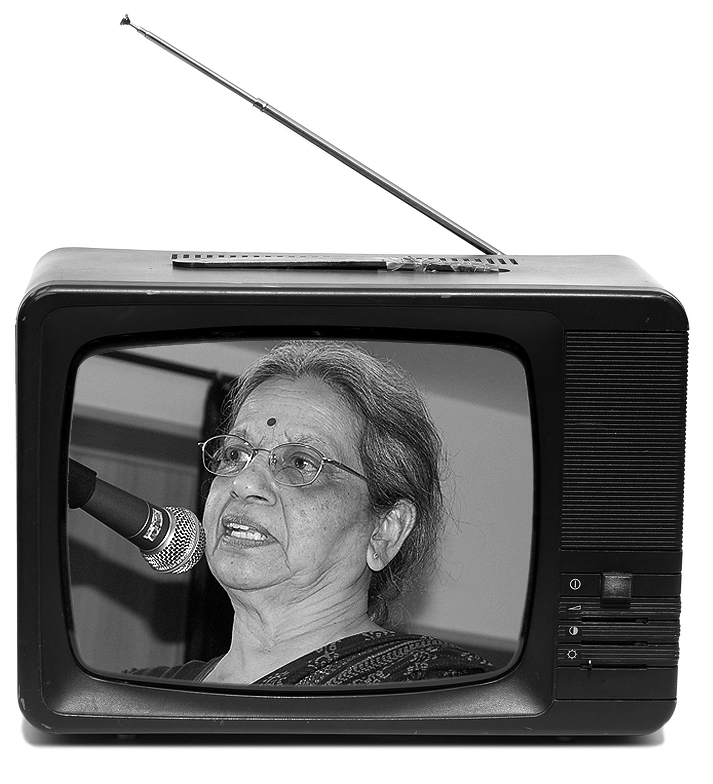
\includegraphics[width=0.4\textwidth,height=4cm]{Kulasthree_Chapter02_pic02.jpg}
\end{center}
\paragraph{}ഇന്ത്യയിലെ സ്ത്രീചരിത്രരചനാരംഗത്തെ ഏറ്റവും പ്രധാനപ്പെട്ട നാമങ്ങളിലൊന്നാണ് ദില്ലി സർവ്വകലാശാലയിൽ പ്രവർത്തിച്ചിരുന്ന ചരിത്രകാരിയായ ഉമാ ചക്രവർത്തിയുടേത്. ഇന്ത്യൻ സമൂഹത്തിൽ ജാതിവ്യവസ്ഥയും സ്ത്രീകളുടെമേൽ നടപ്പിലുള്ള നിയന്ത്രണങ്ങളും തമ്മിലുള്ള അഭേദ്യബന്ധത്തെ സൂക്ഷ്മമായി അപഗ്രഥിക്കുന്നവയാണ് അവരുടെ ചരിത്രപഠനങ്ങൾ. പരമ്പരാഗത ഇന്ത്യൻ സമൂഹത്തിൽ നിലനിന്നിരുന്ന ആൺകോയ്മയെ 'ബ്രാഹ്മണപിതൃമേധാവിത്വം' (brahmanical patriarchy) എന്നാണ് അവർ വിളിക്കുന്നത്. ഇതുപ്രകാരം ഉയർന്ന ജാതികളിൽപ്പെട്ട സ്ത്രീകളെ മേലാളജാതികളുടെ പ്രജനനത്തിനുള്ള ഉപകരണങ്ങളായി കരുതുന്നു. കീഴ്ജാതിസ്ത്രീകളെ ഉയർന്ന ജാതിക്കാർക്കുവേണ്ടി അദ്ധ്വാനിക്കാനും അവരുടെ ലൈംഗികാവശ്യങ്ങൾ നിവർത്തിക്കുന്നതിനായും നിയോഗിക്കുന്നു. ജാതിവ്യവസ്ഥയെ സംരക്ഷിക്കുന്നതിന് മേൽജാതി സ്ത്രീകളെ സമൂഹത്തിൽനിന്ന് ഒഴിച്ചുനിർത്തേണ്ടത് ആവശ്യമാണെന്ന് 'ബ്രാഹ്മണപിതൃമേധാവിത്വ'ത്തിന്റെ വക്താക്കൾ എക്കാലത്തും വാദിച്ചിട്ടുണ്ട്. അന്യജാതിക്കാരുമായി, പ്രത്യേകിച്ച് കീഴ്ജാതിക്കാരായ പുരുഷന്മാരുമായി, അവർ സംസർഗ്ഗത്തിലേർപ്പെട്ടാൽ ഉയർന്നജാതിയുടെ അടിത്തറതന്നെ തകർന്നുപോകുമെന്നുള്ളതുകൊണ്ടാണ് അവരുടെമേൽ വളരെ കടുത്ത നിയന്ത്രണങ്ങൾ ഏർപ്പെടുത്തിയിരുന്നത്. ബ്രാഹ്മണ നിയമവ്യവസ്ഥയും ഇവിടുത്തെ രാജഭരണവും മേൽജാതി സ്ത്രീകൾക്കുമേലുള്ള നിയന്ത്രണങ്ങളെ ന്യായീകരിച്ചു. ആ നിയന്ത്രണങ്ങളെ എതിർത്ത, അല്ലെങ്കിൽ ലംഘിച്ച സ്ത്രീകളെ പുറന്തള്ളാൻ മേൽജാതി സമുദായങ്ങൾ തീരെ മടിച്ചിരുന്നില്ല.}
\end{tcolorbox}
%%%%%%%%%%%

\begin{figure}[h]
\begin{center}
\includegraphics[width=\textwidth,height=9cm]{Kulasthree_Chapter02_pic03.jpg}
\end{center}
\end{figure}

\paragraph{}'ജന്മഭേദവ്യവസ്ഥ'പ്രകാരം ഓരോ ജാതിയിലേയും ആണുങ്ങൾക്കും പെണ്ണുങ്ങൾക്കും വെവ്വേറെ ലിംഗനിയമങ്ങളുണ്ടായിരുന്നു. അതായത് മലയാളബ്രാഹ്മണ (നമ്പൂതിരി) സമുദായത്തിലെ 'ഉത്തമസ്ത്രീസങ്കല്പം' നായർസ്ത്രീകൾക്കോ കീഴ്ജാതിക്കാർക്കോ ബാധകമായിരുന്നില്ല. ഓരോ സമുദായത്തിനും ഇതൊക്കെ പ്രത്യേകം പ്രത്യേകമുണ്ടായിരുന്നു. തീർച്ചയായും അന്നുള്ളവർ ധാരാളം വായിച്ചിരുന്ന പുരാണങ്ങളിലൂടെയും ശീലാവതിചരിതംപോലുള്ള കൃതികളിലൂടെയും ബ്രാഹ്മണരുടെ ലിംഗമൂല്യങ്ങൾ (അതായത്, ആണുങ്ങളായാൽ എങ്ങനെയിരിക്കണം, എന്തു ചെയ്യണം എന്നും പെണ്ണുങ്ങളായാൽ എങ്ങനെയിരിക്കണം, എന്തു ചെയ്യണം എന്നും മറ്റും വിധിക്കുന്ന മൂല്യങ്ങൾ) സമൂഹത്തിൽ പ്രചരിച്ചിരുന്നു. എന്നാൽ, ഇതോടൊപ്പംതന്നെ ഈ മൂല്യങ്ങൾ എല്ലാ സ്ത്രീകൾക്കും ബാധകമല്ലെന്നു സ്ഥാപിക്കുന്ന 'ബ്രാഹ്മണന്യായീകരണങ്ങ'ളും പ്രചരിച്ചിരുന്നുവെന്ന് കാണേണ്ടതുണ്ട്. ഉദാഹരണത്തിന്, കേരളത്തിലെ ശൂദ്രസ്ത്രീകൾ (നായർ-അമ്പലവാസി സമുദായക്കാർ) പാതിവ്രത്യം ആചരിക്കേണ്ടതില്ലെന്ന് കേരളമാഹാത്മ്യം പോലുള്ള ഗ്രന്ഥങ്ങൾ ഉദ്ധരിച്ചുകൊണ്ട് പഴമക്കാർ വാദിച്ചിരുന്നു - ഇവിടത്തെ ശൂദ്രസ്ത്രീകൾ ദേവന്മാരെ ആനന്ദിപ്പിക്കുന്നതിനായി സൃഷ്ടിക്കപ്പെട്ട അപ്സരസ്സുകളുടെ സന്തതികളാണെന്നും അപ്സരസ്ത്രീകൾക്ക് പാതിവ്രത്യം ബാധകമല്ലാത്തതുപോലെ അവരുടെ സന്തതികൾക്കും അതു ബാധകമല്ലെന്നും ഈ കൃതികൾ പറയുന്നു. അതുകൊണ്ട് ശീലാവതിചരിതം വായിച്ചു പുണ്യംസമ്പാദിച്ച നായർസ്ത്രീകൾ ശീലാവതിയെ മാതൃകയാക്കിക്കളയുമെന്ന് പ്രതീക്ഷിക്കേണ്ടതില്ലായിരുന്നു! അതേസമയം ജാതികൾ തമ്മിൽ ലിംഗമൂല്യങ്ങളിൽ കാര്യമായ വ്യത്യാസമുള്ളിടത്ത് ഇവ പലപ്പോഴും വഴക്കിനും കലഹത്തിനും കാരണമായി. ഉദാഹരണത്തിന് തിരുവിതാംകൂറിലെ കരുനാഗപ്പള്ളി-കാർത്തികപ്പള്ളി മേഖലയിൽ (ഓണാട്ടുകരയിൽ) 19-ാം നൂറ്റാണ്ടിൽ നടന്ന ജാതീയ ഏറ്റുമുട്ടലുകളെക്കുറിച്ച് വാമൊഴിയായി പ്രചരിച്ചിട്ടുള്ള കഥകളിൽ പലതിലും വിഷയം മേൽപ്പറഞ്ഞ ലിംഗമൂല്യങ്ങളിലെ പൊരുത്തക്കേടാണ്. മുസ്ലിം സമുദായത്തിലെ സമ്പ്രദായപ്രകാരം സ്ത്രീകൾ നിർബന്ധമായും മേൽവസ്ത്രം ധരിച്ചിരിക്കണം; ഈഴവരുടെയിടയിൽ അക്കാലത്ത് നേരെ തിരിച്ചായിരുന്നു നിയമം - അതായത്, മേൽവസ്ത്രം ധരിച്ചുനടക്കുന്നത് 'നല്ല സ്ത്രീകൾ' ചെയ്യുന്ന പണിയല്ല, 'വേഷംകെട്ടുകാരത്തികളു'ടെ പണിയാണ്! ഈ പ്രദേശത്തെ ചന്തകളിൽ കച്ചവടക്കാര്യത്തിലുംമറ്റും ഈ രണ്ടു സമുദായക്കാർ തമ്മിൽ കടുത്ത മത്സരം നിലനിന്നിരുന്നതുകൊണ്ട് അടികലശലിനുംമറ്റും സാദ്ധ്യതയും കൂടുതലായിരുന്നു. പക്ഷേ, അടി പൊട്ടിപ്പുറപ്പെട്ടത് പലപ്പോഴും വസ്ത്രധാരണത്തെക്കുറിച്ചുള്ള അഭിപ്രായവ്യത്യാസങ്ങളെ ചുറ്റിപ്പറ്റിയായിരുന്നെന്ന് വാമൊഴിക്കഥകൾ സൂചിപ്പിക്കുന്നു. നഗ്നമായ മാറിടവുമായി ചന്തയിലെത്തിയിരുന്ന ഈഴവസ്ത്രീകളെ മുസ്ലീം പുരുഷന്മാർ കളിയാക്കിയെന്നും തുടർന്നു ലഹളയുണ്ടായെന്നുംമറ്റുമാണ് കഥകളിലെ പരാമർശം.


\paragraph{}'ജാതിയിൽ കൂടിയ സ്ത്രീകൾക്ക് കൂടിയ സ്വാതന്ത്ര്യം' എന്ന ഇന്നത്തെക്കണക്ക് അന്ന് എല്ലായിടത്തും ഒത്തിരുന്നില്ലെന്നതാണ് രസകരമായ വസ്തുത. ജാതിയിൽ ഏറ്റവും മുന്തിയവർ എന്ന് സ്വയം അവകാശപ്പെട്ട ബ്രാഹ്മണസ്ത്രീകൾ അതികഠിനമായ നിയന്ത്രണങ്ങൾക്കു വിധേയരായിരുന്നു. അതേസമയം 'താരതമ്യേന സ്വതന്ത്രകൾ' എന്നു നാം തിരിച്ചറിയുന്ന മരുമക്കത്തായ സ്ത്രീകൾ - വിശേഷിച്ചും ഉയർന്ന ജാതിക്കാർ - മറ്റു പലവിധ നിയന്ത്രണങ്ങൾക്കുമുള്ളിലായിരുന്നു. വീട്ടിലെ അദ്ധ്വാനത്തിന്റെ കാര്യമെടുത്താൽ ഉന്നതജാതിക്കാരായ സ്ത്രീകൾപോലും അതിൽനിന്ന് പൂർണ്ണമായും ഒഴിവായിരുന്നില്ലെന്നു വ്യക്തം.

\section{വരേണ്യ മലയാളിസ്ത്രീകളുടെ ദൈനംദിനജീവിതം}
പരമ്പരാഗത മലയാളിസമൂഹത്തിൽ പല ജാതിവിഭാഗങ്ങളിൽപ്പെട്ട സ്ത്രീകളുടെയും സ്ത്രീത്വാദർശവും അവർക്കു ബാധകമായ ദൈനംദിനജീവിതനിയമങ്ങളും വെവ്വേറെയായിരുന്നെന്ന് പറഞ്ഞുവല്ലോ. ഈ വ്യത്യാസത്തിന് ഊന്നൽ നല്കിക്കൊണ്ട്, ലഭ്യമായ വിവരങ്ങൾ അനുവദിക്കുന്നിടത്തോളം പരമ്പരാഗത മലയാളിസമൂഹത്തിലെ പല ജാതിക്കാരായ സ്ത്രീകളുടെ ദൈനംദിനജീവിതം എങ്ങനെയായിരുന്നുവെന്ന് പരിശോധിക്കാനാണ് ഇവിടെ ശ്രമിക്കുന്നത്. എല്ലാ ജാതിക്കാരെക്കുറിച്ചും പറയാൻ സ്ഥലപരിമിതിയും വിവരങ്ങളുടെ കുറവും അനുവദിക്കുന്നില്ല. കേരളത്തിലെ ജാതികളുടെ ആചാരങ്ങൾ, അനുഷ്ഠാനങ്ങൾ, വിവാഹരീതി, വിവാഹകർമ്മം മുതലായവയെക്കുറിച്ച് ധാരാളം വിവരങ്ങൾ നരവംശശാസ്ത്രകൃതികളിൽനിന്നും സർക്കാരിന്റെ ഔദ്യോഗികപ്രസിദ്ധീകരണങ്ങളിൽനിന്നും ലഭ്യമാണ്. ആ വിവരങ്ങൾ ഇവിടെ ആവർത്തിക്കുന്നില്ല.
പരമ്പരാഗത മലയാളിസമൂഹത്തിൽ മേധാവിത്വമുണ്ടായിരുന്ന മലയാള ബ്രാഹ്മണരിൽനിന്നു തുടങ്ങാം. സ്ത്രീകളുടെമേൽ ഏറ്റവും ശക്തമായ നിയന്ത്രണങ്ങൾ ഏർപ്പെടുത്തിയിരുന്ന സമുദായമായിരുന്നു ഇത്. ആൺവഴിക്ക് കുടുംബപിന്തുടർച്ചയും സ്വത്തവകാശവും കണക്കാക്കിയിരുന്നതിനാൽ സ്ത്രീകൾക്ക് കാര്യമായി വിലകൽപിക്കാതിരുന്ന സമൂഹം (എങ്കിലും ഇന്ന് വടക്കേയിന്ത്യയിൽ കാണുന്നത്ര സ്ത്രീവിരുദ്ധത ഇക്കൂട്ടർക്കിടയിൽ ഇല്ലായിരുന്നെന്ന് കരുതാൻ നമ്മെ അനുവദിക്കുന്ന ചില സൂചനകളുണ്ട്). നമ്പൂതിരിയില്ലങ്ങളിൽ ജനനംമുതൽക്കേ ആൺകുട്ടിക്ക് പ്രത്യേക പരിഗണന നൽകുന്ന പല സമ്പ്രദായങ്ങളും പിന്തുടർന്നിരുന്നുവെന്ന് നമ്പൂതിരിസമുദായത്തെക്കുറിച്ച് എഴുതിയ കാണിപ്പയ്യൂർ ശങ്കരൻ നമ്പൂതിരിപ്പാട് പറയുന്നു. പ്രായപൂർത്തിയായിക്കഴിഞ്ഞാൽ പെൺകുട്ടി അന്യപുരുഷന്മാരുമായി സംസാരിച്ചുകൂടാ; എട്ടു വയസ്സുകഴിഞ്ഞാൽ അവൾ വീട്ടുജോലി ചെയ്തുതുടങ്ങണം; കന്യകമാർ നല്ല ഭർത്താവിനെ ലഭിക്കാൻ കഠിനമായ വ്രതങ്ങൾ നോക്കണം - ഇങ്ങനെയൊക്കെയായിരുന്നു നിയമങ്ങൾ. ചേലപ്പുതപ്പുകൊണ്ട് ഉടലാകെ മൂടി, വലിയ മറക്കുടചൂടി, വേലക്കാരുടെ അകമ്പടിയോടെമാത്രമേ നമ്പൂതിരിസ്ത്രീകൾക്ക് (അക്കാലത്ത് മലയാളബ്രാഹ്മണസ്ത്രീകളെ 'അന്തർജനങ്ങൾ' എന്നാണ് വിളിച്ചിരുന്നത്) ഇല്ലംവിട്ട് സഞ്ചരിക്കാൻ അനുവാദമുണ്ടായിരുന്നുള്ളൂ.

\paragraph{}'ഉപനയനം' എന്ന ചടങ്ങുകഴിഞ്ഞാൽ നമ്പൂതിരിബാലന്മാരുടെ ജീവിതവും ദുഃസഹമായിരുന്നെന്ന സൂചന അക്കാലത്തു ജീവിച്ചിരുന്ന പലരുടെയും ആത്മകഥകളിലുണ്ട്. പക്ഷേ, ഈ കഷ്ടപ്പാടിലൂടെ കടന്നുകഴിഞ്ഞാൽ സമുദായത്തിൽ പൂർണ്ണമായ അംഗത്വവും അധികാരവും അവർക്ക് ലഭിക്കുമായിരുന്നു. വാരം, പൂരം തുടങ്ങിയ വിശേഷാവസരങ്ങളിൽ അമ്പലങ്ങളിലും മറ്റു നമ്പൂതിരിയില്ലങ്ങളിലും ഒത്തുകൂടി സദ്യയും വെടിവട്ടവുമായി കഴിയാൻ അവർക്കു കഴിയുമായിരുന്നു. കഷ്ടിച്ച് വായിക്കാൻ പഠിച്ചാൽ അന്തർജനത്തിന്റെ വിദ്യാഭ്യാസം കഴിയും; പിന്നെ വീട്ടിനുള്ളിലും പരിസരത്തുള്ള ഇല്ലങ്ങൾ, അമ്പലങ്ങൾ എന്നിവിടങ്ങളിലും സ്വന്തം വീട്ടിലും മാത്രമായി അവരുടെ ജീവിതം കഴിയും.

\paragraph{}ഇല്ലങ്ങളിലെ അന്തർജനങ്ങളുടെ ദിനചര്യ വളരെ കൃത്യമായി ആവർത്തിക്കേണ്ട ചടങ്ങുകളുടെ നീണ്ട ശൃംഖലതന്നെയായിരുന്നുവെന്നു പറയാം. കുളിപോലും സൂക്ഷിച്ചു ചെയ്യേണ്ട ചടങ്ങുകളുടെ കൂട്ടമായിരുന്നുവെന്ന് കാണിപ്പയ്യൂരിന്റെ വിവരണം വ്യക്തമാക്കുന്നു. അന്തർജനങ്ങൾക്കിടയിൽത്തന്നെ അവിവാഹിതകളായ പെൺകുട്ടികളും വിധവകളുമായിരുന്നു കഠിനവ്രതങ്ങൾ അനുഷ്ഠിച്ചിരുന്നത് - വിധവയെ സംബന്ധിച്ചിടത്തോളം ഭർത്താവിന്റെ മരണശേഷമുള്ള ജീവിതം നീണ്ട ഒരു പ്രായശ്ചിത്തമെന്നോണം ചെലവഴിക്കേണ്ടിവന്നിരുന്നു. ഇല്ലങ്ങളിൽ സ്ത്രീകൾ കൊണ്ടാടിയ അനുഷ്ഠാനപരമായ ആഘോഷങ്ങൾ - തിരുവാതിരയായിരുന്നു അവയിൽ പ്രധാനം - ഭർത്താവിന്റെ ആയുരാരോഗ്യം, ഭർതൃലാഭം, ഭർതൃസുഖം എന്നിവയെ ഉന്നംവയ്ക്കുന്നവയായിരുന്നു. കുടുംബത്തിന്റെ ദൈനംദിന ജീവിതത്തിൽ ഭാര്യയും ഭർത്താവും പരസ്പരം പേർചൊല്ലി വിളിക്കുക, അധികസമയം അടുത്തിരുന്നു സംസാരിക്കുക, കുട്ടികളെ ലാളിക്കുക ഇതൊന്നും പതിവില്ലായിരുന്നുവെന്ന് കാണിപ്പയ്യൂർ ഓർക്കുന്നു; കുട്ടിക്കാലത്ത് മുത്തശ്ശി, ചെറിയച്ഛൻ മുതലായവരാണ് തന്നെ ലാളിച്ചിരുന്നതെന്നും. 
\begin{figure}[h]
\begin{center}
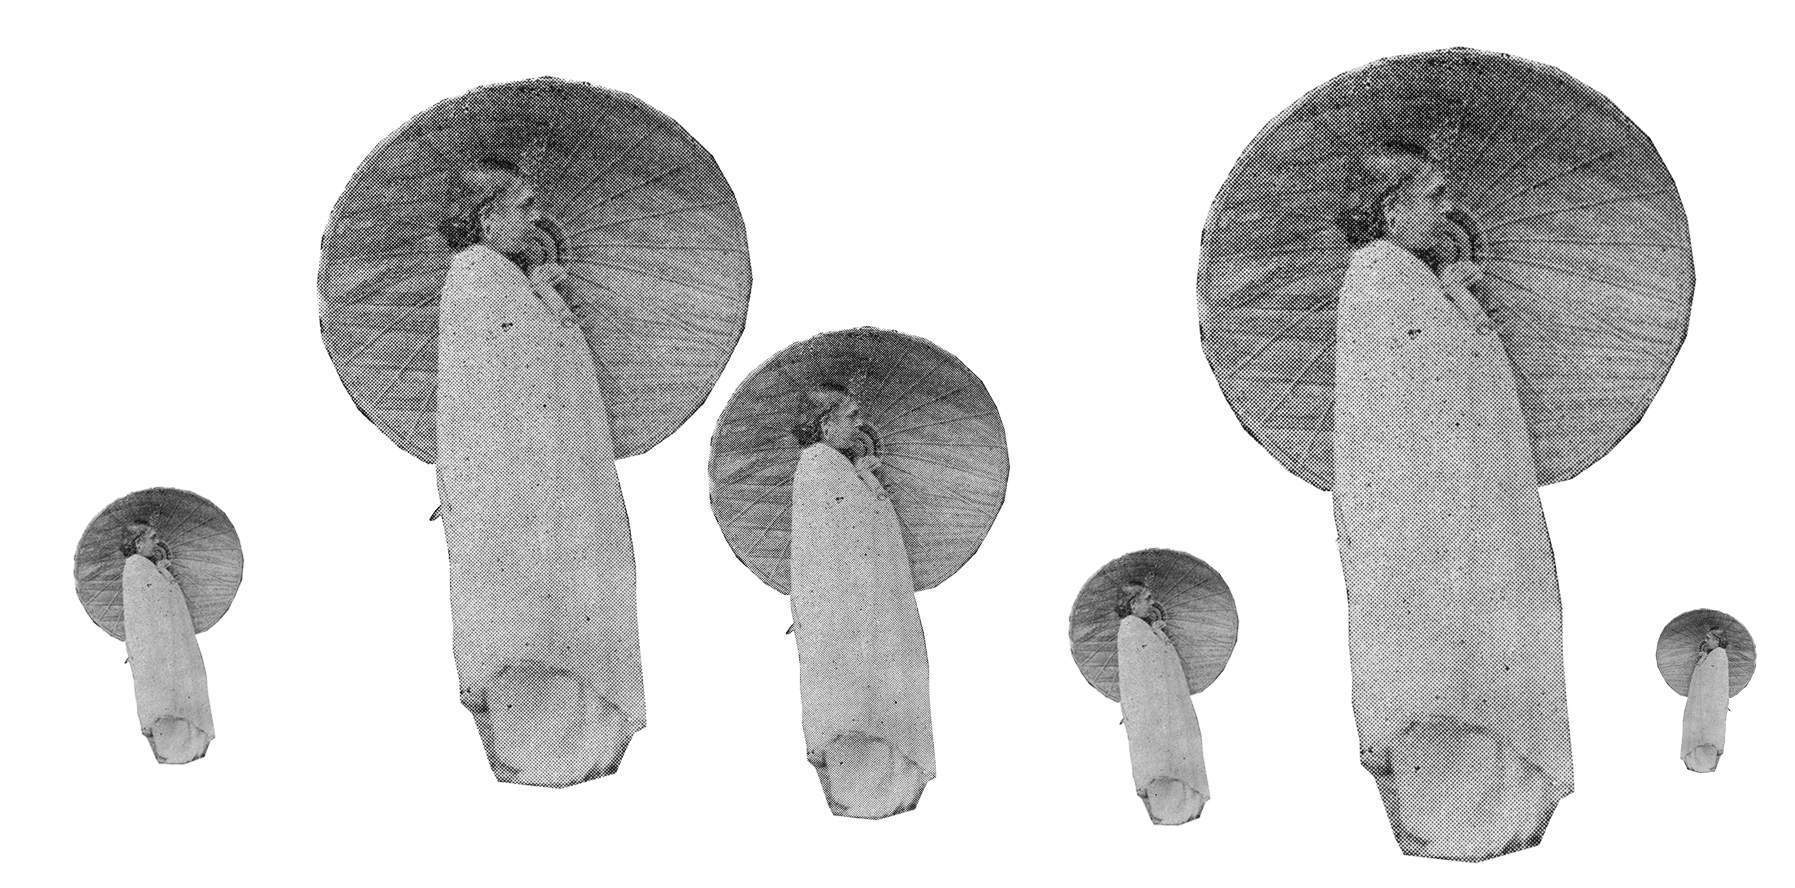
\includegraphics[width=\textwidth,height=10cm]{Kulasthree_Chapter02_pic04.jpg}
\end{center}
\end{figure}

%%%%%BOX%%%%%%
\captionof{mybox}{'മറക്കുടയ്ക്കുള്ളിലെ മഹാനരകം' തിരിച്ചെത്തിയിരിക്കുന്നു!}\label{ch2box2} % place the caption
\begin{tcolorbox}[%
  breakable, % make the box breakable
  arc=0mm, 
  left=1pt, right = 1pt, 
  boxrule=0mm,
  colback = {blue!10}, % since shadow-gray was not defined
] 

\paragraph{}1930കളിലെ നമ്പൂതിരിപരിഷ്ക്കരണപ്രസ്ഥാനത്തിന്റെ ഭാഗമായി അവതരിപ്പിക്കപ്പെട്ട ഒരു നാടകത്തിന്റെ പേരാണിത്. യഥാർത്ഥത്തിൽ നടന്ന ഒരു സംഭവത്തെ ആസ്പദമാക്കിയാണത്രെ എം.ആർ ഭട്ടതിരിപ്പാട് ഈ നാടകമെഴുതിയത്. നമ്പൂതിരിമാരുടെ പരമ്പരാഗത ജീവിതരീതികളിൽ സ്ത്രീകൾക്കു സഹിക്കേണ്ടിവന്ന കടുത്ത അനീതികൾക്കെതിരെ ശബ്ദമുയർത്തുന്ന ഈ നാടകം വലിയ കോളിളക്കമുണ്ടാക്കുകയും ചെയ്തു. അന്യർക്ക് തീരെ അനുവാദമില്ലായിരുന്ന ഇല്ലങ്ങൾക്കുള്ളിലകപ്പെട്ടുപോയ മലയാളബ്രാഹ്മണസ്ത്രീകളെ നിഷ്കരുണം മർദ്ദിക്കാനും അവരുടെ ജീവനെടുക്കാനുംവരെയുള്ള അധികാരം ഭർത്താവിനു നൽകിയിരുന്ന വ്യവസ്ഥയെക്കുറിച്ച് ലോകം അറിയുകയും ചെയ്തു.
\paragraph{}എന്നാൽ, നമ്പൂതിരിയില്ലങ്ങളും മറക്കുടയുംമറ്റും ഇല്ലാതായിക്കഴിഞ്ഞ ഇക്കാലത്തും ഇത്തരം 'മഹാനരകങ്ങ'ളിൽ നാട്ടുകാരോ വീട്ടുകാരോ അറിയാതെ മർദ്ദനം സഹിച്ചു കഴിയുന്ന എത്രയോ സ്ത്രീകളുണ്ട് കേരളത്തിൽ! 'കുടുംബമാന്യത'യെന്ന പുതിയ മറക്കുടയാണ് അവർ ചൂടുന്നത്.
\paragraph{}'ഗാർഹികപീഡനങ്ങളിൽനിന്നും സ്ത്രീകൾക്കുള്ള സംരക്ഷണനിയമം' (Protection of Women from Domestic Violence Act - 2005) നിലവിൽവന്നത് ഈ യാഥാർത്ഥ്യത്തെ അംഗീകരിച്ചുകൊണ്ടാണ്. 'ഗാർഹികപീഡന'ത്തെ വെറും ശാരീരികമായ ദ്രോഹം മാത്രമായിട്ടല്ല ഈ നിയമം കാണുന്നത്. ഒരു വീട്ടിൽ താമസിക്കുന്ന രക്തബന്ധത്തിൽപ്പെട്ടതോ വിവാഹബന്ധത്തിൽപ്പെട്ടതോ അല്ലെങ്കിൽ വിവാഹംമൂലമുള്ള ബന്ധത്തിൽപ്പെട്ടതോ ആയ സ്ത്രീക്ക് ഗൃഹാന്തരീക്ഷത്തിൽ ആ ഗൃഹാന്തരീക്ഷത്തിലെ പ്രായപൂർത്തിയായ ഏതെങ്കിലും പുരുഷനിൽനിന്നുണ്ടാകുന്ന പീഡനത്തെയാണ് ഈ നിയമം 'ഗാർഹികപീഡന'മായി കരുതുന്നത്. ശാരീരികവും ലൈംഗികവും മാനസികവുമായ ഗാർഹികപീഡനത്തെ ഈ നിയമംവഴി നേരിടാനാകും. അതുപോലെ, സ്ത്രീയുടെ തൊഴിലിൽ തടസ്സമുണ്ടാക്കുക, തൊഴിലുപകരണങ്ങൾ നശിപ്പിക്കുക മുതലായ പ്രവൃത്തികളെ 'സാമ്പത്തികപീഡന'മായി കണക്കാക്കുന്ന ഉത്തരവുകളും ഈ നിയമപ്രകാരം പ്രകടിപ്പിക്കപ്പെട്ടിട്ടുണ്ട്. കുടുംബത്തിൽപ്പെട്ട സ്ത്രീകളെ നിരാലംബരാക്കി വഴിയിൽ ഇറക്കിവിടുന്നതും ഈ നിയമം വിലക്കുന്നു - അത്തരം സന്ദർഭങ്ങളിൽ താമസിക്കുന്നതിനുള്ള സംരക്ഷണം ഉറപ്പാക്കുന്നതിനാവശ്യമായ ഉത്തരവു പുറപ്പെടുവിക്കാൻ മജിസ്ട്രറ്റുമാരെ നിയമം അധികാരപ്പെടുത്തുന്നു.

\paragraph{}പരാതിക്കാരി താമസിക്കുന്ന സ്ഥലം, പരാതിക്കു കാരണമായ സംഭവം നടന്ന സ്ഥലം അല്ലെങ്കിൽ എതിർകക്ഷി (പീഡനം നടത്തിയ വ്യക്തി) താമസിക്കുന്ന സ്ഥലം - ഇവയിലേതെങ്കിലുമൊരു സ്ഥലത്തുള്ള ജുഡിഷ്യൽ ഒന്നാംക്ലാസ് മജിസ്ട്രറ്റ് കോടതിയിലാണ് പരാതിപ്പെടേണ്ടത്. ഈ നിയമത്തിൽ പറഞ്ഞിട്ടുള്ള എല്ലാ കാര്യങ്ങളിലും തീരുമാനമെടുക്കാനുള്ള അധികാരം മജിസ്ട്രറ്റിനുണ്ട്. മജിസ്ട്രറ്റിന്റെ ഉത്തരവു ലംഘിക്കുന്നയാൾക്ക് ഒരു വർഷംവരെ തടവ് അല്ലെങ്കിൽ ഇരുപതിനായിരം രൂപവരെ പിഴ അല്ലെങ്കിൽ രണ്ടുംകൂടി നൽകുവാൻ ഈ നിയമം അനുശാസിക്കുന്നു. ഈ നിയമത്തിനുകീഴിൽ ഏറ്റവും മുഖ്യമായ ചുമതലവഹിക്കുന്നയാളാണ് പ്രൊട്ടക്ഷൻ (സംരക്ഷണ) ഓഫീസർ (Protection Officer). ഈ ഓഫീസറാണ് ബന്ധപ്പെട്ട മജിസ്ട്രറ്റിനെ ഗാർഹികപീഡനം നടന്നതോ നടക്കുവാൻ സാദ്ധ്യതയുള്ളതോ തടയാൻ ആവശ്യമുള്ളതോ ആയ കാര്യങ്ങളറിയിക്കേണ്ടത്. പരാതിക്കാരിക്ക് നീതി ഉറപ്പുവരുത്തേണ്ട ചുമതല ഇവർക്കാണ്. ഉത്തരവാദിത്വമില്ലാതെ പ്രവർത്തിക്കുന്ന പ്രോട്ടക്ഷൻ ഓഫീസർമാരെ ശിക്ഷിക്കാനും നിയമത്തിൽ വകുപ്പുണ്ട് - ജാമ്യമില്ലാത്ത കുറ്റകൃത്യങ്ങളുടെ പട്ടികയിലാണ് ഇത് ഉൾപ്പെടുത്തിയിട്ടുള്ളത്. പരാതികൾ വിചാരണയ്ക്കുവരുമ്പോൾ രഹസ്യമായ വിചാരണ (in camera) നടത്തുവാനും വ്യവസ്ഥയുണ്ട്.
(വിവരങ്ങൾക്ക് അഡ്വ. ഗീനാകുമാരിയോടു കടപ്പാട്)
\end{tcolorbox}
%%%%%%%%%%%

\begin{figure}[h]
\begin{center}
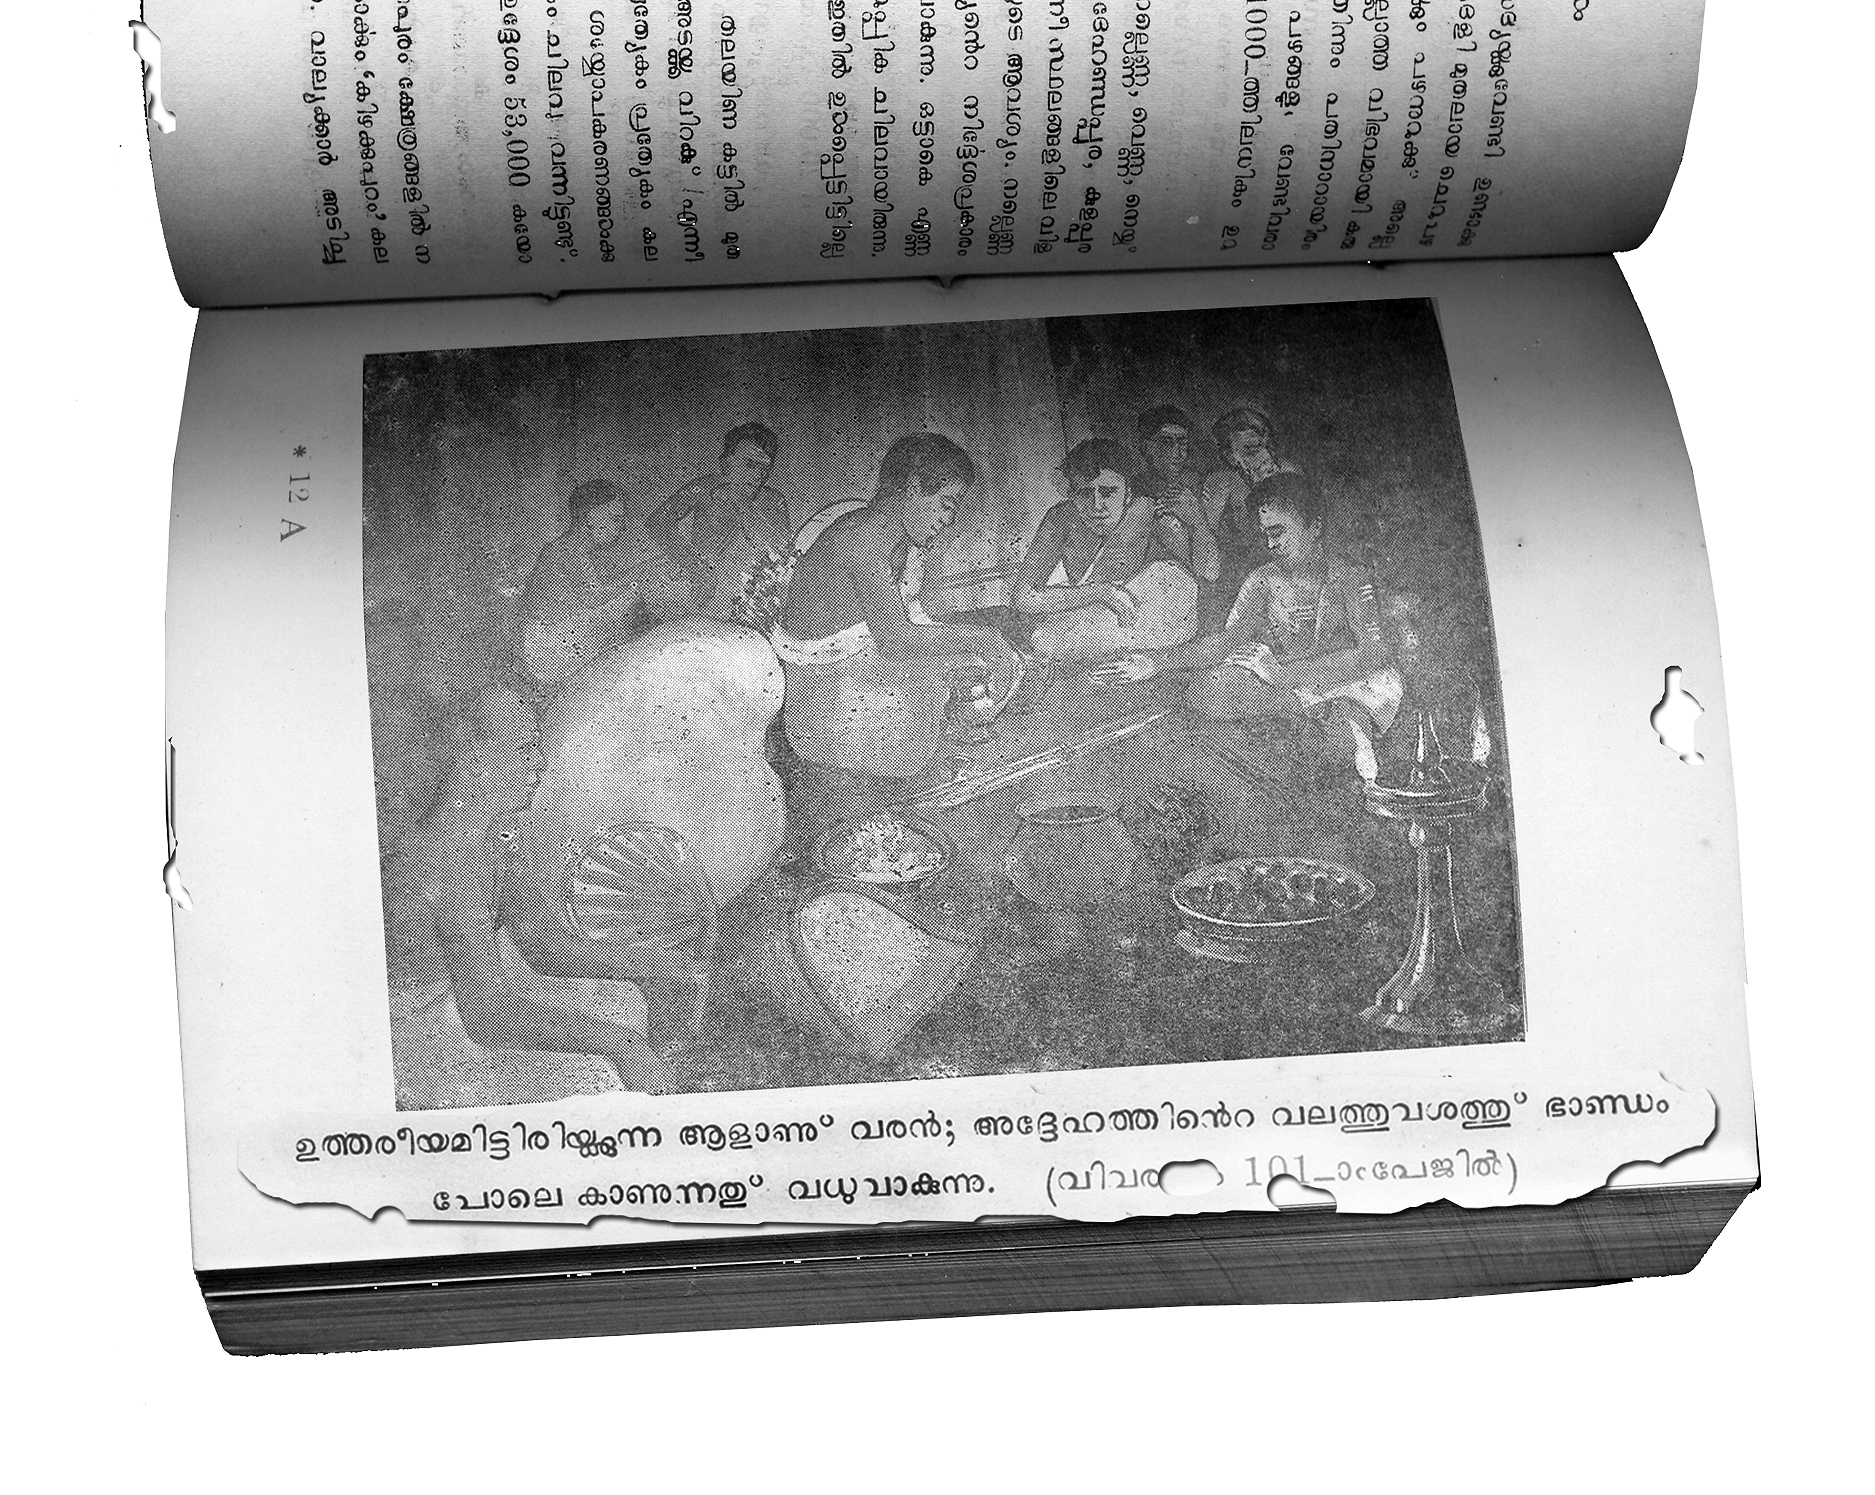
\includegraphics[width=\textwidth,height=6cm]{Kulasthree_Chapter02_pic05.jpg}
\end{center}
\end{figure}


%%%%%BOX%%%%%%
\captionof{mybox}{'പെൺപ്രതിരോധം തെക്കൻപാട്ടുകളിൽ'}\label{ch2box3} % place the caption
\begin{tcolorbox}[%
  breakable, % make the box breakable
  arc=0mm, 
  left=1pt, right = 1pt, 
  boxrule=0mm,
  colback = {blue!10}, % since shadow-gray was not defined
] 

\paragraph{}'പെൺപ്രതിരോധം തെക്കൻപാട്ടുകളിൽ' എന്ന ലേഖനത്തിൽ ടി.ടി. ശ്രീകുമാർ തെക്കൻ തിരുവിതാംകൂറിൽ പ്രബലമായിരുന്ന മരുമക്കത്തായ സമ്പ്രദായം പൊതുവെ സ്ത്രീകേന്ദ്രിതമായിരുന്നുവെന്നും അവ സ്ത്രീകൾക്കു കുറേക്കൂടി അനുകൂലവുമായ സാംസ്കാരികാന്തരീക്ഷം സൃഷ്ടിച്ചിരുന്നുവെന്നും വാദിക്കുന്നു. 'തെക്കൻപാട്ടുകളി'ൽ ഇത് ദൃശ്യമാവുന്നതെങ്ങനെ എന്നു വിശദീകരിച്ചുകൊണ്ടാണ് അദ്ദേഹം ഇങ്ങനെ എഴുതുന്നത്. 'പുരുഷാദേവി' എന്ന പാട്ടിനെക്കുറിച്ച് ജെ. പത്മകുമാരിയുടെ പഠനത്തിൽനിന്ന് അദ്ദേഹം ഉദ്ധരിക്കുന്നു:
\begin{quotation}
%\paragraph{}
\noindent മരുമക്കത്തായ തറവാട്ടിലെ ഭരണവിദഗ്ദ്ധയായ 'കാരണോത്തി'യാണ് പുരുഷാദേവിയെന്നല്ലാതെ, ദ്രാവിഡ-ആര്യ ദേവതകളിലാരോ ആണെന്നു തോന്നുകയേയില്ല. അധികാരദുർമോഹം മുഴുത്ത ഒരുവനായി 'വിമലൻ' പ്രത്യക്ഷപ്പെടുന്നു. അയാളെ പരാജയപ്പെടുത്താൻ എല്ലാശക്തിയും സമാഹരിക്കുകയാണ് ദേവിയുടെ നേതൃത്വത്തിൽ. തെക്കൻ തിരുവിതാംകൂറിലെ മരുമക്കത്തായം 'മിശ്രദായ'മായിരുന്നു. അതായത് പുരുഷന്റെ സ്വത്ത് സ്വന്തം മാതൃകുടുംബത്തിനു പോകുമ്പോഴും വിധവയ്ക്കും മക്കൾക്കും ഒരുഭാഗം ലഭിച്ചിരുന്നു. "പരമ്പരാഗത കേരളത്തിൽ മാതൃദായക്രമം (മരുമക്കത്തായം) നിലവിലിരുന്നുവെങ്കിലും സ്വത്തവകാശം ഇത്തരം കുത്തകവത്ക്കരണത്തെ പ്രതിരോധിക്കുകയും സ്വത്തുവിഭജനം അനിവാര്യമാക്കിത്തീർക്കുകയും ചെയ്തിരിക്കാം".\\ 
\\(ടി.ടി. ശ്രീകുമാർ, ചരിത്രവും ആധുനികതയും, തൃശൂർ, 2001, പുറം. 100)
 \end{quotation}

\end{tcolorbox}
%%%%%%%%%%%

\paragraph{}കുടുംബത്തിലെ മൂത്തമകൻമാത്രം സ്വന്തം സമുദായത്തിൽനിന്ന് വിവാഹംകഴിക്കുകയും ബാക്കിയുള്ള പുരുഷന്മാർ മുഴുവൻ നായർ അമ്പലവാസി സ്ത്രീകളുമായി സംബന്ധത്തിലേർപ്പെടുകയും ചെയ്യുന്ന രീതിയിൽ ഒരു പുരുഷന് പല ഭാര്യമാരുണ്ടായിരുന്നത് സ്വാഭാവികംമാത്രം. പെൺകുട്ടിയെ ഏതുവിധേനയും വിവാഹം കഴിപ്പിക്കേണ്ടതാണെന്ന നിയമവും ഉണ്ടായിരുന്നെന്ന് കാണേണ്ടതാണ് - അവിവാഹിതയായ സ്ത്രീ മരിച്ചാൽ ശവത്തെ താലികെട്ടിച്ച്, ചിലയിടത്ത് കീഴാളപുരുഷന്മാരെ അതിനായി നിയോഗിച്ച്, സംസ്ക്കരിക്കുന്ന രീതിയുണ്ടായിരുന്നു. പ്രായമേറിയ പുരുഷന് നിരവധി ചെറുപ്പക്കാരികളെ ഭാര്യമാരാക്കാൻ കഴിയുമായിരുന്നു. സ്ത്രീധനവും നന്നായി വാങ്ങാനാവുമായിരുന്നു. വിവാഹകാര്യത്തിൽ സ്ത്രീ പുരുഷന് പരിപൂർണ്ണമായും കീഴ്പ്പെട്ടിരുന്നു.

\paragraph{}എന്നാൽ സ്ത്രീകളിൽ ചാരിത്ര്യദോഷം ആരോപിക്കപ്പെട്ടാൽ അവരെ സമുദായത്തിനു പുറത്താക്കാനുള്ള സാദ്ധ്യത അധികവുമായിരുന്നു. 'സ്മാർത്തവിചാരം' എന്നൊരു നീണ്ട പ്രക്രിയയായിരുന്നു ഇത്. ദോഷമാരോപിക്കപ്പെട്ട സ്ത്രീയെ 'അഞ്ചാംപുര' എന്ന പ്രത്യേക മുറിയിലാക്കി (സംശയത്തിൽ കഴമ്പുണ്ടോയെന്ന് അറിയാൻ ഇല്ലത്തെ പണിക്കാരികളെ ചോദ്യംചെയ്യുന്ന 'ദാസീവിചാരം' എന്ന പരിപാടിക്കുശേഷം) അവരെ നീണ്ട ചോദ്യംചെയ്യലിനു വിധേയമാക്കി, കുറ്റസമ്മതം നടത്താതെ സ്ത്രീയെ ഭ്രഷ്ടാക്കാൻ കഴിയില്ലായിരുന്നു; സ്മാർത്തവിചാരം വലിയ ചെലവുള്ള ചടങ്ങായിരുന്നതുകൊണ്ടുതന്നെ അന്തർജനത്തെക്കൊണ്ട് കുറ്റം സമ്മതിപ്പിക്കാൻ കടുത്ത പ്രയോഗങ്ങൾവരെ പലയിടത്തും നടത്തിയിരുന്നത്രെ. കുറ്റം സമ്മതിച്ചാൽ അവളും അവൾ പേരു വിളിച്ചുപറഞ്ഞ പുരുഷന്മാരായ കൂട്ടാളികളും സമുദായത്തിൽനിന്ന് ബഹിഷ്ക്കരിക്കപ്പെടും. ദോഷാരോപിതപുരുഷന്മാർക്ക് തങ്ങളുടെ സാധുത്വം തെളിയിക്കാൻ പല മാർഗ്ഗങ്ങളുമുണ്ടായിരുന്നു - പക്ഷേ, പുറത്തായ അന്തർജനത്തിന് നിരപരാധിത്വം തെളിയിക്കാൻ ഒരു വഴിയും ഉണ്ടായിരുന്നില്ല. \ref{ch10box2}

\paragraph{}രാപ്പകലുള്ള വീട്ടുവേല അന്തർജനങ്ങളുടെ ജീവിതയാഥാർത്ഥ്യമായിരുന്നു. ഇല്ലങ്ങളിൽ വലിയ സദ്യയും മറ്റും നടത്താൻ അന്തർജനങ്ങൾ പണിപ്പെടുന്നതിനെക്കുറിച്ച് 20-ാം നൂറ്റാണ്ടിന്റെ തുടക്കത്തിൽ ചില ലേഖകർ വിവരിച്ചിട്ടുണ്ട്. 1927ലെ നമ്പൂതിരി സ്ത്രീവിദ്യാഭ്യാസക്കമ്മിഷനു മുമ്പാകെ (നമ്പൂതിരിമാരുടെ സമുദായപ്രസ്ഥാനമായ യോഗക്ഷേമസഭയാണ് ഈ കമ്മിഷൻ സ്ഥാപിച്ചത്) തെളിവു നൽകിക്കൊണ്ട് നമ്പൂതിരിപെൺകുട്ടികളെക്കുറിച്ച് മാടമ്പ് നാരായണൻ നമ്പൂതിരി പറഞ്ഞതിങ്ങനെയാണ്:
\begin{quotation}
\noindent ...അധികകാലം പഠിക്കുവാൻ അവർക്കു [അന്തർജനങ്ങൾക്ക്] സമയമില്ല. എട്ടുവയസ്സിൽ അടുക്കളപ്പണിയാരംഭിക്കുന്നു! അടുക്കള മെഴുകുക, പാത്രംതേക്കുക, എച്ചിലെടുക്കുക മുതലായതെല്ലാം അവരുടെ ജോലിതന്നെ. ഇതിന്നു പുറമെ അവരുടെ സഹോദരന്മാരെ 'serve' ചെയ്യേണ്ടതും ഇവരുടെ മുറതന്നെ. ഇങ്ങനെ ഒന്നുരണ്ടുകൊല്ലം കഴിയുമ്പോഴേക്കും അതാ വേറെ ജോലിയുംകൂടി അവരുടെ തലയിൽ വച്ചുകെട്ടുന്നു. അതു മറ്റൊന്നുമല്ല; അന്തർജനഭാഷയിൽ 'നേദിക്കുക'. രാവിലെ മുതൽ 10 മണിവരെ 'നേദിക്കലും' 'നമസ്ക്കാരവും' തന്നെ. കിഴക്കോട്ട്, തെക്കോട്ട്, എന്തിനേറെ എല്ലാ കോണിലേക്കും ഗുരുവായൂരപ്പനും കാവിൽ ശാസ്താവിനും വൈക്കത്തപ്പനും കോവിൽ അയ്യപ്പനും എന്നുവേണ്ട അവർക്കും ഇവർക്കും നേദിക്കൽതന്നെ. ഇതെല്ലാം ആജീവനാന്തം വേണ്ടതുമാണ്... പിന്നെ പകലെ ഉച്ചയ്ക്കുമേൽ രണ്ടുനാഴികയുള്ളതു പുരാണപാരായണത്തിനും 'ചരടുപിടിച്ചു ജപിക്കുന്ന'തിനും ആയി. \\
\\(നമ്പൂതിരി സ്ത്രീവിദ്യാഭ്യാസ കമ്മിഷൻ റിപ്പോർട്ട്, 1928, പുറം 65-66)
\end{quotation}

\paragraph{}എന്താണിതിന്റെ അർത്ഥം? സമുദായത്തിന്റെ മർദ്ദനവും ചൂഷണവുമേറ്റ് തീർത്തും നിഷ്ക്രിയരായിത്തീർന്ന ഒരു വിഭാഗമായിരുന്നു അന്തർജനങ്ങൾ എന്നാണോ? നമ്പൂതിരിസമുദായ പരിഷ്ക്കർത്താക്കളായി 20-ാം നൂറ്റാണ്ടിൽ ഉയർന്നുവന്ന പലരുടെയും രചനകളിൽനിന്ന് ആ തോന്നൽ ഉളവായേക്കാം. 'തട്ടിൽപുറത്ത് വെയിലുകാണാതെ കിടക്കുന്ന ക്ലാവുപിടിച്ച ഓട്ടുപാത്രങ്ങൾ' പോലെയാണ് അന്തർജനങ്ങൾ എന്ന് പ്രസിദ്ധനായ ഒരു സമുദായപരിഷ്കർത്താവ് പ്രഖ്യാപിച്ചിട്ടുമുണ്ട്. പക്ഷേ, 20-ാം നൂറ്റാണ്ടിന്റെ ആദ്യവർഷങ്ങളിലെ പത്രമാസികകൾ പരിശോധിക്കുമ്പോൾ അത്തരമൊരു ചിത്രമല്ല കിട്ടുന്നത്. കടുത്ത നിയന്ത്രണങ്ങൾക്കുള്ളിലാണെങ്കിലും ഇല്ലങ്ങളിലെ സ്ത്രീകൾ ഈ നിയമങ്ങളെ പരോക്ഷമായ രീതിയിൽ ചെറുത്ത സംഭവങ്ങൾ പത്രവാർത്തയായിരുന്നു. ക്രൂരനായ ഭർത്താവിനു കൊടുത്ത വിഷംചേർത്ത പാൽ മകൾ എടുത്തു കുടിച്ചതിനെത്തുടർന്ന് കുറ്റമേറ്റുപറഞ്ഞ അന്തർജനത്തെക്കുറിച്ചും ഉത്സവങ്ങളും കാണാനായി വേഷപ്രച്ഛന്നരായി വീട്ടിൽനിന്ന് രാത്രി പുറത്തുകടക്കുന്ന അന്തർജനങ്ങളെക്കുറിച്ചും മറ്റും വാർത്തകളുണ്ടായിരുന്നു. തങ്ങളെ ബന്ധിച്ച നിയമങ്ങളോട് പൂർണ്ണവിധേയത്വം ഇക്കൂട്ടർക്കില്ലായിരുന്നുവെന്നതിന് തെളിവാണിത്. ഇല്ലങ്ങൾക്കുള്ളിൽ പ്രായക്കൂടുതലിന് കൽപ്പിച്ചിരുന്ന പ്രാധാന്യമാണ് മറ്റൊരു കാര്യം. സ്ത്രീകൾക്ക് ഔദ്യോഗികമായ അധികാരം കുറവായിരുന്നെങ്കിലും മുതിർന്ന സ്ത്രീകൾക്ക് 'അനൗപചാരികമായ അധികാരം' പലപ്പോഴും സ്വന്തമായിരുന്നു. വി.ടി. ഭട്ടതിരിപ്പാടിന്റെ ആത്മകഥയിൽ ഇതു ധാരാളം പ്രത്യക്ഷമാകുന്നുണ്ട്. അടുക്കളയിൽനിന്ന് അരങ്ങത്തേക്ക് എന്ന തന്റെ നാടകം വി.ടിയുടെ ഇല്ലത്ത് അവതരിപ്പിക്കുന്നതിനെ യാഥാസ്ഥിതികനായ ജ്യേഷ്ഠൻ എതിർത്തപ്പോൾ രക്ഷയ്ക്കെത്തിയത് വൃദ്ധയും വിധവയുമായിരുന്ന ഒരു അച്ഛൻപെങ്ങളായിരുന്നത്രെ. വിവാഹനിലയും സ്ത്രീകൾക്ക് 'അനൗപചാരിക അധികാരം' നൽകി - വിധവയും ചെറുപ്പക്കാരിയുമായ ഒരു സ്ത്രീയുടെ നില ദയനീയമായിരുന്നുവെങ്കിൽ, ഭർത്തൃമതിയും ആൺമക്കളുള്ളവളുമായ ഒരു അന്തർജനത്തിന്റെ നില ഭേദമാകാനിടയുണ്ടായിരുന്നു. എന്നാൽ 'അനൗപചാരിക അംഗീകാര'ത്തെ കണക്കറ്റു പുകഴ്ത്തുന്നതിൽ കാര്യമില്ല - കാരണം അത് തീർത്തും ഉറപ്പില്ലാത്ത ഒന്നായിരുന്നു. എത്ര പ്രതാപിയായ മൂത്ത അന്തർജനത്തിന്റെയും 'അനൗപചാരികസ്വാധീനം' ചെറുപ്പക്കാരിയും സുന്ദരിയും മിടുക്കിയുമായ ഒരു സപത്നിയുണ്ടായാൽ ഇളകുന്ന ഒന്നുമാത്രമായിരുന്നു. അതുപോലെ വിധവയായാൽ, ആൺമക്കൾ മരിച്ചാൽ, കുടുംബത്തിൽ അവരുടെ സ്വാധീനം ഇല്ലാതാകുമായിരുന്നു.

\captionof{mybox}{സ്ത്രീപുരുഷന്മാർ ചേർന്നുള്ള വിനോദങ്ങൾ}\label{ch2box4} % place the caption
\begin{tcolorbox}[%
  breakable, % make the box breakable
  arc=0mm, 
  left=1pt, right = 1pt, 
  boxrule=0mm,
  colback = {blue!10}, % since shadow-gray was not defined
] 

\paragraph{}സ്ത്രീകളും പുരുഷന്മാരും ചേർന്നുള്ള നൃത്തം, ഗാനം, വിനോദം മുതലായവ ഇന്ന് കേരളത്തിൽ വിരളമാണ്. (നാടകംപോലുള്ള കലാരൂപങ്ങളുടെ കാര്യമല്ല പറയുന്നത്) എന്നാൽ മുമ്പ് അത്തരത്തിലുള്ള പല വിനോദങ്ങളുമുണ്ടായിരുന്നു. ഓണക്കാലത്തെ പല കളികളിലും ആണുങ്ങളും പെണ്ണുങ്ങളും ഒത്തുചേർന്നിരുന്നു. മദ്ധ്യതിരുവിതാംകൂറിൽ ഓണക്കാലത്ത് അരങ്ങേറിയിരുന്ന 'ഓണത്തുള്ള'ലിൽ സ്ത്രീകളും പുരുഷന്മാരും ഒരുമിച്ച് ആടുകയും പാടുകയും ചെയ്തിരുന്നു. കുരുത്തോലകൊണ്ട് കിരീടമണിഞ്ഞ് സ്ത്രീകളും തുടികൊട്ടിപ്പാടി; പുരുഷന്മാരും ഇതിൽ കൂടിയിരുന്നു. തുമ്പിതുള്ളാനും ആൺകുട്ടികളും പെൺകുട്ടികളും ഒത്തുചേർന്നിരുന്നു. ആലപ്പുഴഭാഗത്ത് 'ആടുകളി' എന്നൊരു വിനോദമുണ്ടായിരുന്നത്രേ! പരസ്പരം 'നോട്ട'മിട്ട ആൺകുട്ടികൾക്കും പെൺകുട്ടികൾക്കും പറ്റിയ അവസരമായിരുന്നു ഇതെന്ന് പഴമക്കാർ പറയുന്നുണ്ട്. ജാതിയുടെ അതിർവരമ്പുകളെ പക്ഷേ, ഇവ അധികമൊന്നും മറികടന്നിരുന്നില്ലെന്നും.
\end{tcolorbox}

\paragraph{}ഇതുമാത്രമല്ല, അന്തർജനങ്ങളുടെ ഒതുങ്ങിക്കൂടിയ ജീവിതശൈലിതന്നെ പലതരം പ്രതിരോധങ്ങൾക്ക് അവസരമൊരുക്കിയിരുന്നു. ഭർത്താക്കന്മാരുടെകൂടെയല്ലാതെ വേലക്കാർക്കൊപ്പമുള്ള സഞ്ചാരം, അങ്ങേയറ്റം സ്വകാര്യമായ അന്തഃപുരങ്ങൾ, ഇതൊക്കെ പലതരം രഹസ്യബന്ധങ്ങൾക്ക് ഇടവരുത്തുമെന്നും നമ്പൂതിരിപുരുഷന്മാർ ജാഗരൂകരാകണമെന്നും 20-ാം നൂറ്റാണ്ടിന്റെ ആദ്യവർഷങ്ങളിൽ മലയാള മനോരമ മുന്നറിയിപ്പു നൽകി. സംബന്ധത്തിനുംമറ്റുമായി നായർവീടുകളിലേക്ക് പുരുഷന്മാർ പുറപ്പെട്ടുകഴിഞ്ഞാൽ വീടുമുഴുവൻ സ്ത്രീകളുടെയും വേലക്കാരുടെയും കൈയിലായിരിക്കുമെന്നും അവർ കൂട്ടുചേർന്ന് സദാചാരവിരുദ്ധ പ്രവൃത്തികളിലേർപ്പെടുമെന്നുമായിരുന്നു പത്രത്തിന്റെ ഭയം. നാട്ടുകാരുടെയും വീട്ടുകാരുടെയും കണ്ണുവെട്ടിച്ച് കാമുകനെ അന്തഃപുരത്തിൽ ഒളിപ്പിച്ചു പാർപ്പിച്ച അന്തർജനത്തെക്കുറിച്ചുള്ള കഥയും അന്നു പത്രവാർത്തയായിരുന്നു. ചുരുക്കിപ്പറഞ്ഞാൽ വളരെ കടുത്ത ബന്ധനങ്ങൾക്കുള്ളിലും ഈ സ്ത്രീകൾ സക്രിയർതന്നെയായിരുന്നു.

\paragraph{}നായർ-അമ്പലവാസി സ്ത്രീകൾ പരമ്പരാഗതവ്യവസ്ഥയിൽ 'അതിസ്വതന്ത്രരാ'യിരുന്നുവെന്നു പറയുന്ന ധാരാളം പുസ്തകങ്ങളുണ്ട്. ബ്രിട്ടിഷ്പൂർവ്വകാലത്തെ പല രേഖകളും ഇതിനെ പിന്താങ്ങുന്നുമുണ്ട്. പല വസ്തുതകളും നമുക്ക് പരിചിതങ്ങളുമാണ്.

\paragraph{}നായർസ്ത്രീക്ക് ഭർത്താവിനെ വേണ്ടെന്നു തോന്നിയാൽ പായചുരുട്ടി പുറത്തുവയ്ക്കണ്ടകാര്യമേ ഉണ്ടായിരുന്നുള്ളൂവെന്നും മറ്റുമുള്ള വിവരണങ്ങൾ എല്ലാവർക്കും അറിയാം. അതുപോലെ മിക്ക കുടുംബങ്ങളിലും പ്രതാപികളായ വല്യമ്മമാരെപ്പറ്റിയുള്ള പഴങ്കഥകളുണ്ട്. ഒറ്റയ്ക്കു കുടുംബത്തെ കടത്തിൽനിന്നു രക്ഷപ്പെടുത്തിയവർ, രാത്രികാലങ്ങളിൽ വിളകൾക്കു കാവൽനിന്നവർ, കിണറ്റിലിറങ്ങി വീണുപോയ തൊട്ടിയെടുത്തവർ, തെങ്ങിൽക്കയറി തേങ്ങയിട്ടവർ - ഇങ്ങനെയൊക്കെ. നായർസ്ത്രീകൾക്ക് സഞ്ചാരസ്വാതന്ത്ര്യവും അന്യപുരുഷന്മാരോട് സംസാരിക്കാനുള്ള സ്വാതന്ത്ര്യവും ഉണ്ടായിരുന്നതായി പറയപ്പെടുന്നു. ഇതിലൊക്കെ വലിയൊരളവുവരെ സത്യവുമുണ്ടായിരുന്നുവെന്നാണ് രേഖകളുടെ സൂക്ഷ്മവായനയിൽനിന്ന് വ്യക്തമാകുന്നത്. പക്ഷേ, അന്തർജനങ്ങൾ 'മൂകരും നിസ്സഹായകളു'മായിരുന്നുവെന്ന സാമാന്യധാരണപോലെത്തന്നെ അതിശയോക്തിപരമല്ലേ നായർ സ്ത്രീകളുടെ 'സ്വാതന്ത്ര്യ'മെന്നും ആലോചിക്കേണ്ടതുണ്ട്. ഒന്നാമത്, ജാതിയുടെ ഉച്ചനീചത്വശ്രണിക്കു കീഴ്പ്പെട്ട സ്വാതന്ത്ര്യമേ അവർക്കുണ്ടായിരുന്നുള്ളു - ജാതിക്കു താഴെയുള്ളവരുമായി സംസർഗ്ഗമുണ്ടായാൽ നായർസ്ത്രീ ജാതിക്കു പുറത്തായിരുന്നു. മദ്ധ്യകാലത്ത് കേരളത്തിൽ നിലവിലുണ്ടായിരുന്ന 'പുലപ്പേടി', 'മണ്ണാപ്പേടി' തുടങ്ങിയ ആചാരങ്ങൾ നായർസ്ത്രീയുടെ 'സ്വാതന്ത്ര്യ'ത്തെ പരിമിതപ്പെടുത്താൻ വേണ്ടിയുള്ളവയായിരുന്നുവെന്ന് ചിലർ വാദിച്ചിട്ടുണ്ട്.

\begin{figure}[h]
\begin{center}
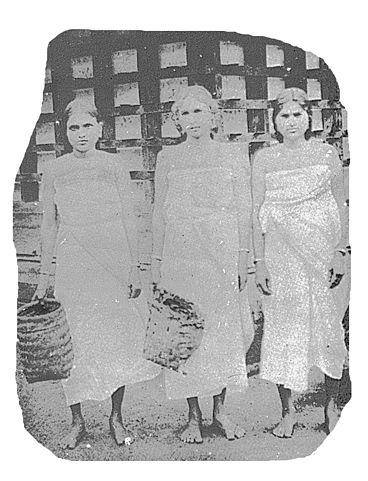
\includegraphics[width=0.7\textwidth,height=8cm]{Kulasthree_Chapter02_pic06.jpg}
\end{center}
\caption*{അമ്പലവാസിസ്ത്രീകൾ - കെ പി പത്മനാഭ മേനോൻ - വാള്യം 3, (1929), 1984}
\end{figure}

\paragraph{}എന്തായാലും 19-ാം നൂറ്റാണ്ടിന്റെ അവസാനകാലത്തും 20-ാം നൂറ്റാണ്ടിലും നായർകുടുംബങ്ങളിലെ സ്ത്രീകളുടെ 'സ്വാതന്ത്ര്യം' പലപ്പോഴും 'കുടുംബ ഉത്തരവാദിത്വത്തിന്റെ ഭാരിച്ച ചുമതല' ആയി മാറിയോ എന്നു സംശയിക്കേണ്ടിയിരിക്കുന്നു. ഇളമുറക്കാർക്ക് ആധുനികവിദ്യാഭ്യാസം നേടിക്കൊടുക്കാനുള്ള തത്രപ്പാടിൽ കുടുംബങ്ങൾ പലതും ക്ഷയിച്ചു. (അതായത് കുടുംബസ്വത്തുക്കൾ വിറ്റും പണയംവച്ചും മറ്റുമാണ് ഇളമുറക്കാരുടെ വിദ്യാഭ്യാസത്തിനുള്ള പണം കാരണവന്മാർ കണ്ടെത്തിയത്). സ്ത്രീകളുടെയും കുട്ടികളുടെയും സാമ്പത്തികസുരക്ഷയെ ഇതെങ്ങനെ ബാധിച്ചുവെന്നതിനെക്കുറിച്ച് അക്കാലത്തും പിൽക്കാലത്തും രചിക്കപ്പെട്ട സാഹിത്യവും ആത്മകഥകളും ധാരാളം പറയുന്നുണ്ട്. കാരണവരുടെ അധികാരങ്ങളെ അരക്കിട്ടുറപ്പിക്കുന്ന നിയമങ്ങൾ ശക്തമായത് സ്ത്രീകളുടെ പരമ്പരാഗത അധികാരങ്ങളെ ബാധിച്ചിരുന്നു. കഴിവില്ലാത്ത കാരണവന്മാരുടെ ഭരണത്തിൻകീഴിൽ പട്ടിണിയെ സമീപിച്ച പല കുടുംബങ്ങളിലും കഠിനമായ അദ്ധ്വാനത്തിലൂടെ കുടുംബം പുലർത്തിയ സ്ത്രീകളെ പല ആത്മകഥകളും ഓർമ്മിക്കുന്നുണ്ട്. പ്രശസ്ത സാഹിത്യകാരൻ പി. കേശവദേവ് എതിർപ്പ് എന്ന തന്റെ ആത്മകഥയിൽ 20-ാം നൂറ്റാണ്ടിന്റെ ആദ്യദശകങ്ങളിൽ കൊച്ചിപ്രദേശത്തു സ്ഥിതിചെയ്തിരുന്ന കൂട്ടുകുടുംബത്തിൽ തന്റെ അമ്മയുടെ ദൈനംദിനജീവിതത്തെക്കുറിച്ച് ഇങ്ങനെ പറയുന്നു:

\begin{quotation}
\noindent നെല്ലുപുഴുങ്ങുക, കുത്തുക, വയ്ക്കുക, വിളമ്പുക, കൃഷിചെയ്യുക മുതലായി നൂറു ജോലികൾക്കിടയിലാണ് കാർത്ത്യായനിയമ്മ പശുക്കളെ ശുശ്രൂഷിക്കുന്നത്. പുല്ലുള്ള സ്ഥലങ്ങൾ കണ്ടുപിടിച്ച് പശുക്കളെ അവിടെക്കൊണ്ടുപോയി കെട്ടുക, ഇടയ്ക്കിടെ അഴിച്ചു മാറ്റിക്കെട്ടുക, കറക്കുക, പാലുകാച്ചുക, തൈരു കലക്കുക, വാങ്ങാൻ വരുന്നവർക്കൊക്കെ യഥാകാലം കൊടുക്കുക, അതെല്ലാം കാർത്ത്യായനിയമ്മതന്നെ ചെയ്യണം... (പുറം. 23)\\

\noindent... കാർത്ത്യായനിയമ്മ രാവുംപകലും പണിയെടുക്കും. പറമ്പിലെല്ലാം അവർതന്നെ കൃഷിചെയ്യും. കാച്ചിലും കിഴങ്ങും വഴുതനയും പടവലവും മറ്റും. അവർതന്നെ കിളയ്ക്കും; അവർതന്നെ നടും; അവർതന്നെ വളമിടും; അവർതന്നെ വെള്ളം കോരും. എല്ലാം പറിച്ചുകൊണ്ടുവന്നു വേവിച്ചാൽ എല്ലാവർക്കുമായി പങ്കിട്ടുകൊടുക്കും... ഉണങ്ങിവീഴുന്ന ഓലയെല്ലാം കാർത്ത്യായനിയമ്മ വെള്ളത്തിലിട്ട് മെടഞ്ഞു വിൽക്കും. പുളിയും പിന്നയ്ക്കായും പറിച്ചുവിറ്റ് കാശാക്കും... കാരണവർ ചെലവിനു തരുന്നതിനുപുറമേ അരിവാങ്ങാൻവേണ്ടിയാണ് അവർ അതെല്ലാം വിൽക്കുന്നത്... (പുറം. 65)

\end{quotation}

\paragraph{}പഴയതിൽനിന്നു പുതിയതിലേക്കുള്ള മാറ്റത്തിനിടയിൽ സ്ത്രീകളുടെ വീട്ടദ്ധ്വാനം വളരെയധികം വർദ്ധിക്കുകയുമുണ്ടായി. വിദ്യാലയങ്ങൾ, സർക്കാർ ഓഫീസുകൾ, കോടതികൾ മുതലായ സ്ഥലങ്ങളിലേക്ക് ജോലിക്കും പഠിപ്പിനും മറ്റുമായി പുരുഷന്മാർ പോയിത്തുടങ്ങിയപ്പോൾ അവരുടെ ആഹാരരീതി, വസ്ത്രധാരണം മുതലായവയിലും മാറ്റം വന്നു. ചോറുപൊതി കൊണ്ടുപോവുക, അലക്കിത്തേച്ച വസ്ത്രം ധരിക്കുക മുതലായ ആവശ്യങ്ങൾ കൂടുതലായി പ്രത്യക്ഷപ്പെട്ടുതുടങ്ങിയതോടെ സ്ത്രീകളുടെ അടുക്കളപ്പണിയെയും മറ്റു വീട്ടുജോലികളെയും കൂടുതൽ ചിട്ടപ്പെടുത്തേണ്ടതായി വന്നു. പ്രശസ്ത സാഹിത്യകാരനായ തകഴി ശിവശങ്കരപ്പിള്ള തന്റെ ആത്മകഥയിൽ (എന്റെ ബാല്യകാലകഥ, തൃശൂർ, 1967) തന്റെ തറവാട്ടിലെ സ്ത്രീകൾക്ക് 'സൺലൈറ്റ്' സോപ്പ് വിപണിയിലെത്തിയതോടെ അതിനോടുണ്ടായ താല്പര്യത്തെക്കുറിച്ച് ഓർമ്മിക്കുന്നുണ്ട്. അതു വരുംമുമ്പ് മുണ്ട് അലക്കി വെളുപ്പിക്കുക എന്ന ജോലി വളരെ ശ്രമകരമായിരുന്നു. എന്നാൽ സോപ്പുവന്നതോടെ ആ പണി എളുപ്പമായി; അതു വാങ്ങണമെന്ന് സ്ത്രീകൾ നിർബ്ബന്ധം പിടിച്ചുതുടങ്ങി. സ്ത്രീകളുടെ മടിയല്ല വാസ്തവത്തിൽ ഈ നിർബന്ധത്തിൽനിന്നു വായിക്കേണ്ടത്. ഇരുപതാം നൂറ്റാണ്ടിന്റെ ആരംഭദശകങ്ങളിൽ (തകഴിയുടെ ബാല്യകാലത്ത്) പുരുഷന്മാർ പുറത്തുപോകുമ്പോൾ സ്വീകരിച്ച വസ്ത്രധാരണരീതി വളരെ മാറിയിരുന്നുവെന്ന് നാം ഓർക്കേണ്ടതുണ്ട്. പുറത്തുപോകുമ്പോൾ അവർ പാലിക്കേണ്ടിയിരുന്ന ശുചിത്വ മാനദണ്ഡങ്ങളും വേറെയായിക്കഴിഞ്ഞിരുന്നു. ജോലിഭാരമേറിയപ്പോൾ അതിനോടു പൊരുത്തപ്പെടാനുള്ള വഴിയെന്ന നിലയ്ക്കാവാം ഒരുപക്ഷേ, സ്ത്രീകൾ സോപ്പു വാങ്ങണമെന്ന് ആവശ്യപ്പെട്ടത്.

\begin{figure}[h]
\begin{center}
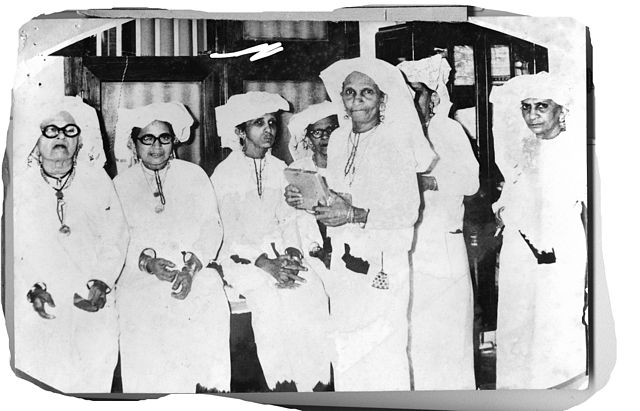
\includegraphics[width=\textwidth,height=10cm]{Kulasthree_Chapter02_pic07.jpg}
\end{center}
\caption*{പി. പി മമ്മതു കോയ, 1994}
\end{figure}

\captionof{mybox}{മാപ്പിളസ്ത്രീകൾ/മുസ്ലിം സ്ത്രീകൾ വെറും 'അടിമ'കളായിരുന്നോ?}\label{ch2box5} % place the caption
\begin{tcolorbox}[%
  breakable, % make the box breakable
  arc=0mm, 
  left=1pt, right = 1pt, 
  boxrule=0mm,
  colback = {blue!10}, % since shadow-gray was not defined
] 

\paragraph{} സാമ്പ്രദായികചരിത്രരചന പലപ്പോഴും പ്രചരിപ്പിച്ചിട്ടുള്ള ഒരു വാർപ്പുമാതൃക (stereotype)യാണിത്. എന്നാൽ മുസ്ലീം സ്ത്രീകളുടെ ചരിത്രത്തെക്കുറിച്ച് നടന്നുവരുന്ന പുതിയ അന്വേഷണങ്ങൾ ഇതിന്റെ അടിത്തറ ഇളക്കിക്കൊണ്ടിരിക്കുന്നു. മുൻകാലങ്ങളിൽ കേരളത്തിലെ മുസ്ലീങ്ങൾക്ക് സുപരിചിതമായിരുന്ന അറബിമലയാളഭാഷയിൽ (മലയാള അക്ഷരങ്ങളെ സമാനമായ അറബിലിപികളിൽ എഴുതുന്ന രീതി) എഴുതാനും വായിക്കാനും മുസ്ലിം സ്ത്രീകൾ പഠിച്ചിരുന്നുവെന്നും, അവർ മതാദ്ധ്യായനം നടത്തിയിരുന്നെന്നും ഷംഷാദ് ഹുസൈൻ, ബി.എസ്. ഷെറിൻ തുടങ്ങിയ സ്ത്രീചരിത്രഗവേഷകർ ചൂണ്ടിക്കാണിക്കുന്നു. ഷംഷാദ് ഹുസൈൻ പറയുന്നു:

\begin{quotation}
\noindent ഇങ്ങനെ സാമ്പ്രദായികവിദ്യാഭ്യാസം നേടുകയും വായിക്കുകയും പാടുകയും പഠിപ്പിക്കുകയും ചെയ്തുകൊണ്ട് അവൾ [മാപ്പിളമുസ്ലിം സ്ത്രീ] സമുദായത്തിനകത്ത് ലഭ്യമായ ഇടത്തെ പ്രയോജനപ്പെടുത്തിയിരുന്നതായി കാണാം. മുഖ്യധാരാമൂല്യങ്ങളിലാണ് ഇവർ വിവരംകെട്ടവരായത്. അടുക്കളയിൽ ഒതുങ്ങിക്കഴിയുന്ന, നിർവാഹകത്വം ഇല്ലാത്ത, ഇരകൾ ആയിത്തീരുന്നത്. (പുറം.15) ബീവിമാരെന്നപേരിൽ ദിവ്യശക്തിയുണ്ടെന്ന് വിശ്വസിക്കപ്പെട്ട സ്ത്രീകളുണ്ടായിരുന്നു - തിരുവനന്തപുരത്തെ ബീമാപള്ളിയും പൊന്നാനിയിലെ ഇബ്രാഹിമാബീവിയുടെ പേരിലുള്ള പള്ളിയും പ്രശസ്തമാണ് എന്ന് ഷംഷാദ് ചൂണ്ടിക്കാട്ടുന്നു (പുറം. 18). മാത്രമല്ല, സ്ത്രീകൾ എഴുതിയ മാപ്പിളപ്പാട്ടുകളിൽ വളരെ ശക്തമായ പിതൃമേധാവിത്വവിരുദ്ധനിലപാടും താൻപോരിമയും ദൃശ്യമാണെന്ന് അവർ പറയുന്നു. പുത്തൂർ ആമിനയുടെ കത്തുപാട്ടിനെ അവർ ഉദാഹരണമായി പറയുന്നു: "ഒരു കേഡിയോട് ഇടഞ്ഞുനിൽക്കാനുള്ള ചങ്കൂറ്റം മാത്രമല്ല ഇതിലുള്ളത് [ആമിനയുടെ കത്തുപാട്ടിൽ]. സ്ത്രീയുടെ സ്വതന്ത്രമായ തെരഞ്ഞെടുപ്പ്, പുരുഷകേന്ദ്രിതമായ കുടുംബഘടനയോടുള്ള വിമർശനം തുടങ്ങിയവയെല്ലാം ഇതിൽ സൂചിതമായിട്ടുണ്ട്." (പുറം 25). "പുത്തൂർ ആമിനയെക്കൂടാതെ ബി. ആയിശക്കുട്ടി, പി.കെ. ഹലീമ, സി.എച്ച്. കുഞ്ഞയിശ തുടങ്ങിയവരും മാപ്പിളപ്പാട്ടുരചയിതാക്കൾ എന്ന നിലയിൽ ശക്തമായ സാന്നിദ്ധ്യം അറിയിച്ചിരുന്നവരാണ്" (പുറം 23). കാണുക \ref{ch9sec1} \\
\\(ഷംഷാദ് ഹുസൈൻ, ന്യൂനപക്ഷത്തിനും ലിംഗപദവിക്കുമിടയിൽ, തിരുവനന്തപുരം, 2009)

\end{quotation}
\end{tcolorbox}

\paragraph{}നായർതറവാടുകളിൽ മുതിർന്ന സ്ത്രീകൾക്ക് അധികാരവും അംഗീകാരവും സ്വാതന്ത്ര്യവും ഉണ്ടായിരുന്നെങ്കിൽ, 20-ാം നൂറ്റാണ്ടിലെ സാമ്പത്തികക്കുഴപ്പം (1920കളുടെ ഒടുക്കംമുതൽ) മൂർച്ഛിച്ചതോടെ (പലപ്പോഴും അതിനുമുമ്പും) അവരുടെ ഭാരങ്ങളും വർദ്ധിച്ചുവെന്നർത്ഥം.(കാണുക \ref{chapter5})കാരണവരോടുള്ള വിധേയത്വം വാക്കിലും നോക്കിലും പ്രവൃത്തിയിലും പാലിക്കേണ്ടിയിരുന്ന സ്ത്രീകൾ, പക്ഷേ, പരമ്പരാഗതമായ തങ്ങളുടെ അവകാശങ്ങൾ നിഷേധിക്കപ്പെടുന്ന വേളകളിൽ എല്ലായ്പ്പോഴും നിഷ്ക്രിയരായിരുന്നില്ല. കാരണവർ തറവാട്ടിലെത്തുന്ന ദിവസം പെണ്ണുങ്ങളാരും ഉറക്കെ ചിരിച്ചുകൂടാ; ഏറ്റവും മുതിർന്ന സ്ത്രീപോലും വാതിൽക്കൽ മറഞ്ഞുനിന്നേ എന്തെങ്കിലും പറയാവൂ എന്നൊക്കെയായിരുന്നു നിയമങ്ങൾ. എന്നാൽ കാരണവർ നൽകുന്ന തുക ഒന്നിനും തികയാതെവരുമ്പോൾ കുടുംബാവശ്യത്തിനുവേണ്ടി പറമ്പിൽനിന്നെടുക്കാൻ സ്ത്രീകൾ ഒട്ടും മടിച്ചിരുന്നില്ല. കേശവദേവ് ഇത് ഓർക്കുന്നുണ്ട്:
\begin{quotation}
\noindent...കാരണവരില്ലാത്ത തക്കംനോക്കി കാർത്ത്യായനിയമ്മ തൈത്തെങ്ങുകളിൽ ആക്രമണം നടത്തും. തോട്ടിയിൽ അരിവാൾ വച്ചുകെട്ടി തേങ്ങാ അറുത്തിടും. അരയ്ക്കാനും വിറ്റ് ഉപ്പുംമുളകും മറ്റും വാങ്ങാനുംവേണ്ടിയാണ് ഇതു ചെയ്യുന്നത്... തേങ്ങാ വെട്ടാൻ കണക്കന്മാർ പറമ്പിൽ വന്നാലുടൻ... അടുക്കളയുടെ അടുത്തുള്ള തെങ്ങുകളിൽനിന്ന് തേങ്ങാ വെട്ടിയിടുമ്പോഴാണ് സ്ത്രീകളുടെ മോഷണം നടക്കുന്നത്. സ്ത്രീകളുള്ളതുകൊണ്ട്, കാരണവർ അങ്ങോട്ടെങ്ങും പോവുകയില്ല. തേങ്ങാക്കുല ചിതറിവീഴുമ്പോൾ, അടുക്കളയിലും ചാമ്പലിലും എച്ചിൽക്കുഴിയിലും വിറകിന്റെ ഇടയിലും എല്ലാം രണ്ടും മൂന്നും വീതം എടുത്തു തള്ളിക്കളയും... (പുറം 25)

\end{quotation}

\paragraph{}പരിചയമില്ലാത്തവരുമായി സംസാരിക്കുന്നതിനുംമറ്റും നായർസ്ത്രീകളുടെമേൽ വലിയ നിയന്ത്രണമുണ്ടായിരുന്നില്ലെന്ന പ്രസ്താവവും കൂടുതൽ സൂക്ഷ്മമായി പരിശോധിക്കേണ്ടതാണ്. ആഭിജാത്യം കൂടുതലുണ്ടെന്ന് കരുതപ്പെട്ട തറവാടുകളിലെ സ്ത്രീകൾ കൂടുതൽ നിയന്ത്രണത്തിനു വിധേയരായിരുന്നു; ആഭിജാത്യം കുറഞ്ഞവർക്ക് അത് താരതമ്യേന കുറവും. കുടുംബവീടുകൾക്കുള്ളിൽ പുരുഷന്മാരും സ്ത്രീകളും തമ്മിലുള്ള തരംതിരിവ് വ്യക്തമായിരുന്നു. നമ്പൂതിരി ഇല്ലങ്ങളിലെ അവഗണന ഇവിടെ സ്ത്രീകൾ സഹിച്ചിരുന്നില്ല, എങ്കിലും പുരുഷന്മാരും സ്ത്രീകളും തറവാട്ടുവീടിന്റെ പ്രത്യേകം ഭാഗങ്ങളിലാണ് തങ്ങിയിരുന്നത്. കുട്ടികളെ വളർത്തുന്ന കാര്യത്തിൽ സ്ത്രീകളും പുരുഷന്മാരും ഏകദേശം തുല്യ ഉത്തരവാദിത്വം വഹിച്ചു - ആൺകുട്ടികൾ ഒരു പ്രായത്തിനുശേഷം അമ്മാവന്മാരുടെയോ അച്ഛന്റെയോ ശിക്ഷണത്തിലായി. പെൺകുട്ടികൾ അമ്മ - കുഞ്ഞമ്മ - വല്യമ്മമാരുടെകൂടെയും. ഇല്ലങ്ങളിലെന്നപോലെ ധനസ്ഥിതിയുള്ള നായർതറവാടുകളിലും പണിക്കാർക്ക് കുട്ടികളെ വളർത്തുന്നതിൽ വലിയ പങ്കുണ്ടായിരുന്നു. പ്രായംകുറഞ്ഞ സ്ത്രീ മിക്ക കാര്യങ്ങളിലും പ്രായംകൂടിയ സ്ത്രീക്ക് വിധേയയായിരുന്നു.


\captionof{mybox}{`പുലപ്പേടി'}\label{ch2box6} % place the caption
\begin{tcolorbox}[%
  breakable, % make the box breakable
  arc=0mm, 
  left=1pt, right = 1pt, 
  boxrule=0mm,
  colback = {blue!10}, % since shadow-gray was not defined
] 

\paragraph{}

കേരളം സന്ദർശിച്ച മദ്ധ്യകാലസഞ്ചാരികൾമുതൽ പലരും വർണ്ണിച്ച ആചാരമായിരുന്നു 'പുലപ്പേടി'. വർഷത്തിൽ ഒരു പ്രത്യേകസമയത്ത് - ചിലയിടത്ത് കർക്കടകമാസത്തിൽ - സൂര്യാസ്തമയത്തിനുശേഷം വീട്ടിനുപുറത്തുവച്ച് ഏതെങ്കിലും ഉന്നതജാതിക്കാരിയായ സ്ത്രീയെ പുലയർ സ്പർശിക്കാനിടവന്നാലോ പുലയർ എറിഞ്ഞ കല്ല് അവരുടെ ദേഹത്തുകൊണ്ടാലോ അവർ ജാതിയിൽനിന്ന് പുറത്താവുകയും പുലയജാതിക്കാരുടെ സ്വന്തമാവുകയും ചെയ്തിരുന്നത്രെ. ഈ സമയത്ത് പുലയജാതിക്കാർ ഒളിഞ്ഞിരുന്ന് നായർസ്ത്രീകളെ സ്പർശിക്കാൻ ശ്രമിക്കുമായിരുന്നത്രെ. അങ്ങനെ സ്പർശിക്കപ്പെട്ടാൽ ആ സ്ത്രീ ഉടനടി ഏതെങ്കിലും പുലക്കുടിയിൽ അഭയംപ്രാപിക്കുമായിരുന്നത്രെ. സ്വന്തം കുടുംബക്കാരുടെ കൊലക്കത്തിയിൽനിന്ന് രക്ഷപ്പെടാൻ! ഒറ്റയ്ക്കു താമസിക്കാനും മറ്റും തയ്യാറായിരുന്ന നായർസ്ത്രീകളെ മെരുക്കാനുള്ള ഒരു സമ്പ്രദായമായിരുന്നു ഇതെന്ന് ചിലർ അഭിപ്രായപ്പെട്ടിട്ടുണ്ട്. 1696ൽ തിരുവിതാംകൂറിൽ കേരളവർമ്മ പുലപ്പേടി നിരോധിച്ചുകൊണ്ട് കല്പന പുറപ്പെടുവിക്കുകയുണ്ടായി. പുലപ്പേടി നിരോധിച്ചതിനെതിരെ ഒരു പുലയകലാപം നടന്നുവെന്നും അത് അടിച്ചമർത്തപ്പെട്ടുവെന്നും വിവരിക്കുന്നുണ്ട്, 'വലിയകേശിക്കഥ' എന്ന തെക്കൻപാട്ടിൽ.
\end{tcolorbox}

\captionof{mybox}{പൊയ്കയിൽ അപ്പച്ചൻ}\label{ch2box7} % place the caption
\begin{tcolorbox}[%
  breakable, % make the box breakable
  arc=0mm, 
  left=1pt, right = 1pt, 
  boxrule=0mm,
  colback = {blue!10}, % since shadow-gray was not defined
] 

\paragraph{}

ഇരുപതാംനൂറ്റാണ്ടിൽ കേരളത്തിലെ കീഴാളജനങ്ങളുടെ രോദനത്തെയും രോഷത്തെയും ഗാനമായും കവിതയായും പൊതുജനങ്ങൾക്കിടയിൽ അവതരിപ്പിച്ച കീഴാളനേതാവും ഗുരുവുമായിരുന്നു പൊയ്കയിൽ അപ്പച്ചൻ. പൊയ്കയിൽ യോഹന്നാൻ, ശ്രീ കുമാര ഗുരുദേവൻ എന്നീ പേരുകളിൽ അദ്ദേഹത്തെ ജനങ്ങൾ ഇന്നും ആരാധിക്കുന്നു. തിരുവല്ലയ്ക്കടുത്തുള്ള ഇരവിപേരൂരിൽ 1879ൽ പൊയ്കയിൽവീട്ടിൽ കുഞ്ഞുളേച്ചിയുടെയും മല്ലപ്പള്ളി പുതുപറമ്പിൽ കണ്ടന്റെയും മകനായി അദ്ദേഹം ജനിച്ചു. സ്ഥലത്തെ പ്രധാനപ്പെട്ട ഒരു സുറിയാനി ക്രിസ്ത്യാനിക്കുടുംബത്തിന്റെ അടിയാളരായിരുന്നു അദ്ദേഹത്തിന്റെ മാതാപിതാക്കൾ. കീഴാളജനങ്ങളുടെ ജീവിതത്തിന്റെ കയ്പുമുഴുവൻ കുടിച്ചുകൊണ്ടായിരുന്നു ബാല്യകാലം. സുവിശേഷപ്രചരണത്തിലൂടെ മതപരിവർത്തനം നടത്താൻ ഇംഗ്ലണ്ടിൽനിന്ന് പത്തൊമ്പതാം നൂറ്റാണ്ടിൽ കേരളത്തിലേക്കു വന്ന സി.എം.എസ്. മിഷണറിമാരുടെ സ്വാധീനം അവിടങ്ങളിൽ ശക്തമായിരുന്നു. അങ്ങനെ ബാല്യകാലത്തുതന്നെ മിഷണറിപ്പള്ളിക്കൂടത്തിൽ അദ്ദേഹം എഴുത്തുപഠിച്ചു. 'കുമാരൻ' എന്ന പേര് 1891ൽ മതംമാറിയതോടെ 'യോഹന്നാൻ' എന്നാക്കി. അസാമാന്യ വാഗ്പാടവമുണ്ടായിരുന്ന യോഹന്നാൻ സുവിശേഷപ്രചാരകനായി വളരെക്കാലം ശോഭിച്ചു - പക്ഷേ, അദ്ദേഹം ബൈബിളിനെക്കുറിച്ചു മാത്രമായിരുന്നില്ല പറഞ്ഞിരുന്നത് - അടിമസന്തതികളുടെ അവസ്ഥയെക്കുറിച്ചും ഉദ്ബോധനം നടത്തിക്കൊണ്ടിരുന്നു. ക്രിസ്തീയസമുദായത്തിനുള്ളിലെ ജാതീയ ഉച്ചനീചത്വങ്ങൾ അദ്ദേഹത്തെ അലട്ടി. ഒടുവിൽ മാർത്തോമാസഭ വിട്ടുപോകാൻതന്നെ അദ്ദേഹം തീരുമാനിച്ചു; മിഷണറിസഭകളുമായുള്ള ബന്ധവും വിച്ഛേദിച്ചു. ഇതോടെ അദ്ദേഹത്തിന്റെ ശത്രുക്കൾ പെരുകി; ജീവനുതന്നെ ഭീഷണിയുയർന്നു. എല്ലാത്തിനെയും മറികടന്ന് അദ്ദേഹം പ്രവർത്തനം തുടർന്നു. ക്രമേണ 'പ്രത്യക്ഷരക്ഷാദൈവസഭ' എന്ന പുതിയ വിശ്വാസസഭയ്ക്ക് 1910ൽ രൂപംകൊടുത്തു. തിരുവിതാംകൂർ ഭരണാധികാരികൾ അദ്ദേഹത്തിന്റെ പ്രവർത്തനങ്ങളെ അനുഭാവപൂർവ്വം വീക്ഷിച്ചു. 1921ലും 1931ലും അദ്ദേഹം ശ്രീമൂലം പ്രജാസഭയിലേക്ക് നാമനിർദ്ദേശം ചെയ്യപ്പെട്ടു - അടിമസന്തതികളുടെ മുഴുവൻ പ്രതിനിധിയായി. അവിടെ കീഴാളർക്കു വിദ്യാഭ്യാസസൗകര്യങ്ങൾ നേടിയെടുക്കാനും അവർക്ക് ഭൂമി ലഭ്യമാക്കാനും അദ്ദേഹം പ്രവർത്തിച്ചു. 1939ൽ അന്തരിച്ചു. അദ്ദേഹത്തിന്റെ വിശ്വാസപ്രമാണങ്ങൾ ഇന്നും പ്രസക്തമായിത്തന്നെ തുടരുന്നു. അപ്പച്ചന്റെ ഗാനങ്ങളിൽനിന്ന്:
\begin{quote}{}
താതനെ ഒരിടത്തും\\
മാതാവെ വേറിടത്തും\\
കുട്ടികളനാഥരായതും\\
മറപ്പതാമോ\\
അടിമ മറപ്പതാമോ...\\
...അപ്പനെയൊരിടത്തും\\
അമ്മയെ വേറിടത്തും\\
സന്താനങ്ങളങ്ങുമിങ്ങും\\
അലഞ്ഞു വിളിച്ചു\\
മാനത്തു പറക്കുന്ന\\
എന്റെ ചക്കിപ്പരുന്തേ\\
നീ പോകും ദിക്കു ദേശത്തെ\\
ഞങ്ങളുടെ അമ്മയെക്കണ്ടോ?\\
ഒരു വാമൊഴി ചൊല്ലിപ്പോയ\\
അപ്പനെക്കണ്ടോ?\\
\\(പി.പി സ്വാമി, ഇ.വി. അനിൽ (സമ്പാദകർ), പൊയ്കയിൽ അപ്പച്ചന്റെ പാട്ടുകൾ 1905-1939, 2006, പുറം 20)
\end{quote}
\end{tcolorbox}

\begin{figure}[h]
\begin{center}
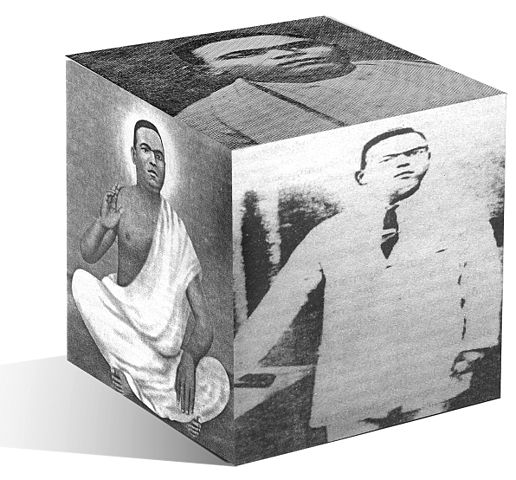
\includegraphics[width=\textwidth,height=8cm]{Kulasthree_Chapter02_pic08.jpg}
\end{center}
%\caption*{പി. പി മമ്മതു കോയ, 1994}
\end{figure}

\captionof{mybox}{അടിമത്തത്തിൽ എന്തു സ്വാതന്ത്ര്യം?}\label{ch2box8} % place the caption
\begin{tcolorbox}[%
 breakable, % make the box breakable
  arc=0mm, 
  left=1pt, right = 1pt, 
  boxrule=0mm,
  colback = {blue!10}, % since shadow-gray was not defined
] 

\paragraph{}
അടിമയായ കീഴാളസ്ത്രീയുടെ 'സ്വാതന്ത്ര്യം' നമ്മെ പരിഹസിച്ചു പല്ലിളിക്കുന്ന കാഴ്ചയാണ് പൊയ്കയിൽ അപ്പച്ചന്റെ ഗാനങ്ങളിൽ കാണുന്നത്. അടിമത്ത നിരോധനം യാഥാർത്ഥ്യമായപ്പോൾമാത്രമാണ് ആ സ്വാതന്ത്ര്യത്തിന് അല്പമെങ്കിലും അർത്ഥമുണ്ടായത്. എന്നിട്ടും തമ്പുരാക്കന്മാരുടെ ക്രൂരതകൾക്കു വിധേയരായ അവരുടെ സ്വാതന്ത്ര്യം അധികവും നിരർത്ഥകമായിരുന്നു. അപ്പച്ചന്റെ ഒരു ഗാനത്തിൽ ഒരു അടിമസ്ത്രീയുടെ വിലാപം:\\
\begin{quote}
.. ഞാനുമെന്റെ കണവനും\\
ഏറെനാൾ താമസം ചെയ്തു\\
ഏഴുകുട്ടി ജനിച്ചതും മറപ്പതല്ല\\
മൂത്തജാതൻ പിറന്നോരു\\
സമയം നാമിരുവരും\\
ആർത്തിപൂണ്ടങ്ങിരുന്നല്ലോ എൻ കണവനേ\\
കാലമേറെ ചെല്ലും മുമ്പേ\\
മീനമാസം കിളച്ചപ്പോൾ\\
ജാതനാം മൂത്തകുട്ടിയെ ഉറുമ്പരിച്ചു\\
അടി ഇടി ഏറ്റുപിന്നെ\\
ഹേമദണ്ഡം ഏറ്റു പിന്നെ\\
രണ്ടാം കുട്ടി ജനിച്ചപ്പോൾ സങ്കടം മാറി\\
ഇരുവരും വേല ചെയ്താൽ\\
അഷ്ടിക്കണ്ടില്ലാത്ത നേരം\\
പാടത്തിൽപോയി ഭക്ഷണങ്ങൾ തിരക്കിയല്ലോ\\
ഒരുനേരം വേല ചെയ്വാൻ\\
കഴിവില്ലാതിരുന്നപ്പോൾ\\
ഉടനേ തമ്പുരാൻ കൊല ചെയ്‌വാനായി വന്നു\\
അരുകിൽ നിദ്രയാലെ\\
ഉറങ്ങിക്കിടന്ന മകളെ\\
മറന്നെൻ ജീവനെതേടിപോയ മകളേ\\
നിന്റെ തള്ള എവിടെപ്പോയ്\\
എന്നു ചൊല്ലി അടിച്ചതാൽ\\
പൊടിമണ്ണിനോടു ചേർന്നു മരിച്ചോ മകളെ\\
ആരോടു ഞാൻ പറയേണ്ടു\\
എങ്ങോട്ടു ഞാൻ പോയിടേണ്ടു\\
ഒട്ടുമേ സഹിപ്പതല്ല മൽപ്രിയ സഖിയേ\\
....\\
പിന്നീടിരു കുട്ടികളോ ഞാൻ\\
വേലയ്ക്കായി പോയനേരം\\
കടുവയാൽ പിടിക്കപ്പെട്ടു മരിച്ചുപോയി\\
ശേഷിച്ച മൂന്നു കുട്ടികൾ\\
ചേലോടു വളർന്നുവന്നു\\
സങ്കടം തീരുവാനായ് തുടങ്ങിയപ്പോൾ\\
നാളിതഞ്ചാറാകുന്നല്ലോ\\
എന്നുടെ കണവനാകും\\
ചോതിയെ വിറ്റ സ്ഥലം ഞാൻ അറിയുന്നില്ല\\
വാങ്ങിയവനെന്നെ കൊണ്ടു\\
പോകുവാനായ് തുടങ്ങുമ്പോൾ\\
കെട്ടിക്കുടിപ്പിച്ചു ഞാൻ കരഞ്ഞീടുന്നു.\\
കുളിപ്പിച്ചേ മകനേ ഞാൻ\\
ചോറു കൊടുത്തല്ലലോടെ\\
അവസാനത്തുരുളയും നീയുണ്ടോടാ മകനേ\\
മൂത്തകുട്ടി കണ്മണിയേ\\
പിരിഞ്ഞു ഞാൻ പോയിടട്ടേ\\
കുട്ടികളേ രണ്ടിനേയും നീ പോറ്റുമോ മകനേ...\\
\\(വി.വി. സ്വാമി, ഇ.വി. അനിൽ (സമ്പാദകർ) പൊയ്കയിൽ അപ്പച്ചന്റെ പാട്ടുകൾ, 1905-1939) കോട്ടയം, 2006, പുറം. 19-20)
\end{quote}
\end{tcolorbox}

\paragraph{}സഞ്ചാരസ്വാതന്ത്ര്യകാര്യത്തിലും സൂക്ഷ്മപരിശോധന ആവശ്യമുണ്ട്. കേരളത്തിന്റെ പല ഭൂഭാഗങ്ങൾക്കും അതിരിട്ടിരുന്ന നദികൾ കടന്നാൽ ശൂദ്രസ്ത്രീ (ബ്രാഹ്മണ-ക്ഷത്രിയ-വൈശ്യ-ശൂദ്രരടങ്ങിയ വർണ്ണവ്യവസ്ഥപ്രകാരം നായന്മാർ 'ശൂദ്രവർണ്ണ'ത്തിൽ ഉൾപ്പെട്ടവരായിരുന്നു) ഭ്രഷ്ടാകുമെന്ന വിശ്വാസം 19-ാം നൂറ്റാണ്ടിന്റെ അവസാനംവരെയും പലയിടത്തും ശക്തമായിരുന്നു. വടക്കേ മലബാറിൽ സ്ത്രീകൾ കോരപ്പുഴ കടക്കരുതെന്നായിരുന്നു നിയമം. ഇംഗ്ലീഷ് വിദ്യാഭ്യാസം നേടിയ നായർ പുരുഷന്മാരെ ഇതു വെട്ടിലാക്കിയെന്നും ഈ നിബന്ധന ബാധകമല്ലായിരുന്ന നായർ ഉപജാതികളിലെ സ്ത്രീകളെ അവർ വിവാഹമാലോചിക്കുന്നുവെന്നും 20-ാം നൂറ്റാണ്ടിന്റെ ആരംഭകാലത്ത് മലബാറിൽ ഗവേഷണം നടത്തിയ നരവംശശാസ്ത്രജ്ഞൻ ഫ്രെഡ്ഫാസറ്റ് (Fred Fawcett) പറയുന്നു. മാസമുറ വന്നതിനുശേഷം 'ശുദ്ധ'മാകണമെങ്കിൽ മണ്ണാത്തിയുടെ കയ്യിൽനിന്ന് 'മാറ്റ്' വാങ്ങണമെന്ന വിശ്വാസവും നായർസ്ത്രീയുടെ ചലനസ്വാതന്ത്ര്യത്തെ ബാധിച്ചു. (മാസമുറ കഴിഞ്ഞാൽ കുളിച്ചു ശുദ്ധമായശേഷം മണ്ണാത്തി - അലക്കുകാരി - അലക്കിയെടുത്ത വസ്ത്രം ധരിക്കുന്നതിനാണ് 'മാറ്റ്' എന്നു പറഞ്ഞിരുന്നത്. മാറ്റു കിട്ടാനിടയില്ലാത്ത നാട്ടിലേക്കു പോകാൻ നായർസ്ത്രീകൾക്കു സമ്മതമില്ലായിരുന്നത്രെ!). (കാണുക \ref{chapter11}).

\paragraph{}മരുമക്കത്തായ കൂട്ടുകുടുംബത്തിലെ മുതിർന്ന സ്ത്രീകൾ അനുഭവിച്ചിരുന്ന അധികാരത്തെക്കുറിച്ചുള്ള കഥകളോട് സാമ്യംപുലർത്തുന്ന പല കഥകളും മക്കത്തായ സമുദായമായ സുറിയാനി ക്രിസ്ത്യാനികൾക്കിടയിലുമുണ്ട്. ഈ അധികാരം തികച്ചും അനൗദ്യോഗികമായിരുന്നെന്നുമാത്രം. മൂത്തസ്ത്രീകൾക്ക് ഇളയസ്ത്രീകളുടെമേൽ അതിശക്തമായ നിയന്ത്രണാധികാരമുണ്ടായിരുന്നുവെന്ന് 19-ാം നൂറ്റാണ്ടിൽ കോട്ടയത്ത് പ്രവർത്തിച്ചിരുന്ന സി.എം.എസ് മിഷണറി ആയിരുന്ന ശ്രീമതി കോളിൻസ് രചിച്ച ഘാതകവധം (1877) എന്ന നോവൽ സൂചിപ്പിക്കുന്നു. സുറിയാനി കുടുംബങ്ങളുടെ ദൈനംദിന ജീവിതത്തിലേക്ക് ധാരാളം ഉൾക്കാഴ്ചകൾ നൽകുന്ന ഈ കൃതിയിൽ ചെറുപ്പക്കാരിയും വിദ്യാസമ്പന്നയുമായ മറിയത്തെ തനിയാഥാസ്ഥിതികയായ ഒരു സ്ത്രീ പെണ്ണുകാണുന്ന ഒരു രംഗമുണ്ട്:
\begin{quotation}
\noindent... ഇടുങ്ങിയ നോട്ടത്തോടും അതൃപ്തിഭാവത്തോടുംകൂടിയ ഒരു ചെറിയ സ്ത്രീ വന്നു മറിയത്തിന്റെ തലയിൽക്കിടന്ന കവണി പുറകോട്ടു വലിച്ചു... അവൾ മറിയത്തിന്റെ അടിക്കാതിൽ വിരലിട്ടുകൊണ്ട് അരികെ നിന്നിരുന്ന അവളുടെ അമ്മയോടു പറഞ്ഞു - "ഇതു കൊച്ചായിപ്പോയി..." ഇത്രയും പറഞ്ഞത് ഒരു ഉറച്ച വല്ലാത്ത ശബ്ദത്തോടുകൂടിയായിരുന്നു... ഇതിന്റെശേഷം അവൾ തലക്കെട്ടേൽ പിടിച്ചു പറഞ്ഞു, ഹൊ ഇതും തുലോം ചെറുതായിപ്പോയി.... വായും നല്ലകണക്കല്ല...\\
\\(ഘാതകവധം, കോട്ടയം (1877), 1996, പുറം. 108)
\end{quotation}
\begin{figure}[h]
\begin{center}
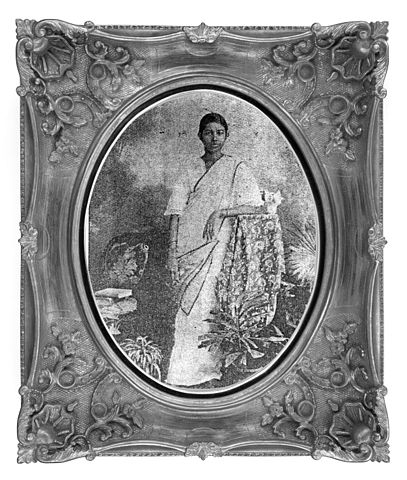
\includegraphics[width=0.7\textwidth,height=8cm]{Kulasthree_Chapter02_pic09.jpg}
\end{center}
%\caption*{പി. പി മമ്മതു കോയ, 1994}
\end{figure}


ഈ സ്ത്രീ അമ്മായിയമ്മയായാൽ തന്റെ ഗതി എന്താകും എന്നോർത്ത് മറിയം ദുഃഖിച്ചു.
\begin{quotation}
\noindent ആ സ്ത്രീ എന്നെക്കൊണ്ടു ചെയ്യിക്കുന്ന വേലകൾ ഒന്നുകിൽ വൈകുന്നതുവരെ നെല്ലുകുത്ത്, അല്ലെങ്കിൽ പറമ്പിൽ അടിച്ചുവാരുകയും വെള്ളംകോരുകയും ചട്ടിയും കലവും തേച്ചുമെഴക്കുകയും ആയിരിക്കും. ഞാൻ വച്ചാൽ വിശേഷമെന്ന് എന്റെ അമ്മ സമ്മതിക്കുന്ന ആ നല്ല കറികൾ അവരെന്നെക്കൊണ്ടു വയ്പിക്കയില്ല. ഞാൻ മോരുകാച്ചിയാൽ എന്റെ അപ്പനു പെരുത്ത് ഇഷ്ടംതന്നെയെങ്കിലും അതും എന്നെക്കൊണ്ട് ചെയ്യിക്കുവാൻ അവർക്കു വിശ്വാസമില്ലായിരിക്കും... (പുറം. 109)
\end{quotation}

\paragraph{}സാഹിത്യകൃതിയിലെ ഈ പരാമർശത്തെ സ്ഥിരീകരിക്കുന്ന നരവംശശാസ്ത്ര പഠനം 20-ാം നൂറ്റാണ്ടിൽ ഉണ്ടായിട്ടുണ്ട്. അമ്മായിയമ്മ എല്ലായ്പ്പോഴും ദുഷ്ടകഥാപാത്രമൊന്നുമല്ലെങ്കിലും മരുമകളുടെമേൽ അവർക്കു സമ്പൂർണ്ണാധികാരമുണ്ടായിരുന്നുവെന്ന കാര്യത്തിൽ യാതൊരു സംശയവുമില്ല. ഈ അധികാരം അടുത്തകാലത്തും നിലനിന്നുവെന്നാണ് സമീപകാലത്തുണ്ടായ പഠനങ്ങൾ സൂചിപ്പിക്കുന്നത്. സാമൂഹ്യശാസ്ത്രജ്ഞയും സാഹിത്യകാരിയുമായ സൂസൻ വിശ്വനാഥൻ യാക്കോബാ സമുദായത്തെക്കുറിച്ചു നടത്തിയ പഠനത്തിൽ ചേർത്തിട്ടുള്ള ഒരു അഭിമുഖത്തിൽ ഒരാൾ ഇതേക്കുറിച്ചു പറയുന്നുണ്ട്:
\begin{quotation}
\noindent പഴയകാലത്തെ പ്രശ്നം ശണ്ഠക്കാരിയായ അമ്മായിയമ്മയല്ല, ശണ്ഠക്കാരിയായ മരുമകളായിരുന്നു. അനുസരണയും കണ്ടുപഠിക്കാനുള്ള മനസ്സുമുള്ള ഒരു ചെറുപ്പക്കാരിയാന്നെങ്കിൽ, [വിവാഹത്തിന്റെ] ആദ്യത്തെ 3-4 വർഷം വളരെ വിലപ്പെട്ട വിദ്യാഭ്യാസം ആർജ്ജിക്കേണ്ട കാലമാണ്. പക്ഷേ, ഈ സമയത്ത് യാതൊരു സ്വാതന്ത്ര്യവും കാണില്ല; അതു പ്രതീക്ഷിക്കാനും വയ്യായിരുന്നു. പറഞ്ഞതുപോലെ ചെയ്തേ പറ്റൂ; സ്വന്തമിഷ്ടത്തിനൊന്നും സ്ഥാനമില്ല. അക്കാലത്തു കുടുംബം വലുതായിരുന്നു; ഒരുപാടു പണിക്കാരുണ്ടാവും; ഒരുപാട് വിരുന്നുകാർ വരും. എല്ലാവർക്കും ആഹാരം കൊടുത്തശേഷമേ പെണ്ണുങ്ങൾ ഉണ്ണാനിരിക്കൂ. ജോലിക്കൂടുതൽകൊണ്ട് ഊണുകഴിക്കാതെ കഴിച്ചുകൂട്ടേണ്ടിവരുന്ന ദിവസങ്ങളുമുണ്ടായിരുന്നു. അമ്മായിയമ്മ ചോറുതന്നില്ല എന്നൊന്നും പരാതിപ്പെട്ടിട്ടു കാര്യമൊന്നുമുണ്ടാവില്ല! ഇതൊക്കെ കുടുംബജീവിതത്തിൽ പ്രതീക്ഷിക്കേണ്ട കാര്യങ്ങൾ മാത്രമായിരുന്നു.\\
\\(Susan Viswanathan, The Christians of Kerala: History, Belief, and Ritual among the Yakoba, New Delhi, 2003, പുറം.115)
\end{quotation}
\paragraph{}കഠിനാദ്ധ്വാനത്തിനുപുറമെ ആചാരാനുഷ്ഠാനങ്ങളിലുള്ള നിഷ്ഠയും യാഥാസ്ഥിതിക സുറിയാനി കുടുംബങ്ങളിൽ കാണാനുണ്ടായിരുന്നെന്നും അതു പാലിക്കുന്നത് സ്ത്രീകളുടെ ഉത്തരവാദിത്വമായിരുന്നെന്നും സൂചനയുണ്ട്. 1922ൽ പി.കെ. കൊച്ചീപ്പൻ തരകൻ പ്രസിദ്ധീകരിച്ച ബാലികാസദനം എന്ന നോവൽ കുടുംബപാരമ്പര്യത്തെ മുറുക്കിപ്പിടിച്ച 'നല്ല സ്ത്രീ'യായ അന്നമ്മയുടെ കുടുംബഭരണത്തെ ഇങ്ങനെ വർണ്ണിക്കുന്നു:
\begin{quotation}
\noindent അതിരാവിലെ നനച്ചുകുളി, ആഴ്ചയിൽ രണ്ടു തേച്ചുകുളി, ചാണകംതളി, 'കോലമിടീൽ' മുതലായ പലതും സൂര്യന്റെ ഗതിക്കു ഭേദമുണ്ടായാൽ മാത്രമെ ആലുംമൂട്ടിലും ഭേദപ്പെടുകയുള്ളൂ. അടുക്കളയിൽ താനല്ലാതെ മറ്റാരും പ്രവേശിച്ചുകൂടാ. അടുക്കള സാമാനങ്ങളിൽ 'അജ്ഞാനികളും' അടുത്തകാലത്തു മാർഗ്ഗംകൂടിയ ക്രിസ്ത്യാനികളും തൊട്ടുകൂടാ. മുറ്റത്താരും തുപ്പിക്കൂടാ. മണ്ണെണ്ണവിളക്കു കൊളുത്തുകയില്ല. നമസ്ക്കാരവും, നോമ്പും കുമ്പസാരങ്ങളും മുടങ്ങുകയില്ല.\\
\\(ബാലികാസദനം, തൃശൂർ, (1922), 1992, പുറം 64 )
\end{quotation}
\paragraph{}മരുമക്കത്തായമായാലും മക്കത്തായമായാലും പൊതുവിൽ ചില കാര്യങ്ങളുണ്ടെന്ന് ഇതുവരെയുള്ള ചർച്ചകളിൽനിന്ന് വ്യക്തമാകുന്നു. ഒന്ന്, വരേണ്യസമുദായങ്ങളിലെ കൂട്ടുകുടുംബങ്ങളിൽ സ്ത്രീകൾ അനുഭവിച്ചിരുന്ന 'അനൗപചാരിക അധികാര'ത്തെക്കുറിച്ചാണ്. ഔപചാരിക അധികാരം സ്ത്രീകൾക്ക് കൽപ്പിക്കാത്ത സമുദായങ്ങളിലും സ്ത്രീകൾക്ക് 'അനൗപചാരിക അധികാരം' ഉണ്ടായിരുന്നു. എന്നാൽ ഈ അധികാരത്തിന് ഉറപ്പില്ലായിരുന്നു - അതുകൊണ്ട് വരേണ്യകുടുംബത്തിലെ വൃദ്ധസ്ത്രീകളെ 'ശക്തിസ്വരൂപിണികളാ'യോ 'ഗൃഹചക്രവർത്തിനിമാരാ'യോ ചിത്രീകരിക്കുന്ന രീതി പുനഃപരിശോധിക്കേണ്ടതാണ്. പ്രായവും സ്ഥാനവും അധികാരവും തമ്മിലുള്ള ബന്ധമാണ് രണ്ടാമത്തെ കാര്യം. പ്രായക്കൂടുതലുള്ള സ്ത്രീക്ക് കൂടുതൽ 'നിലയും വിലയും' രണ്ടു വ്യവസ്ഥകളിലുമുണ്ടായിരുന്നു. സ്ഥാനത്തിനും അത്രതന്നെ പ്രാധാന്യമുണ്ടായിരുന്നു. മൂന്നാമത്തെ കാര്യം, അദ്ധ്വാനത്തെക്കുറിച്ചാണ്. ഉന്നതജാതിക്കാരായ സ്ത്രീകൾ - വലിയ പ്രഭുകുടുംബത്തിൽ പിറക്കാത്തവർ - വീട്ടിനുള്ളിലും വീടിനുചുറ്റും നന്നായി അദ്ധ്വാനിച്ചിരുന്നുവെന്ന് നാം കണ്ടു. അല്പം സാമ്പത്തികശേഷിയും 'മഹിമ'യും സമ്പാദിച്ചുകഴിഞ്ഞാൽ 'തറവാട്ടുകാരികൾ' വീടിനുചുറ്റും അദ്ധ്വാനിക്കാത്ത രീതി താരതമ്യേന സമീപകാലത്തുണ്ടായതാണെന്ന് വ്യക്തം - പഴയ കുടുംബങ്ങളിലെ സ്ത്രീകൾ കൃഷിയിലും മൃഗസംരക്ഷണത്തിലുംമറ്റും മുഴുകിയിരുന്നു. പൊതുവെ പറഞ്ഞാൽ വീട്ടിനുള്ളിൽ അദ്ധ്വാനിച്ച അന്തർജനങ്ങളൊഴികെ മറ്റു സ്ത്രീകൾ വീടിനുചുറ്റും അദ്ധ്വാനിച്ചിരുന്നു; നായർ-ഈഴവർ തുടങ്ങിയ മരുമക്കത്തായ സമുദായക്കാരികൾക്ക് മറ്റുള്ളവരോട് സംസാരിക്കാനും മറ്റും തടസ്സങ്ങളില്ലായിരുന്നു. മലബാറിലെ മാപ്പിള-മുസ്ലീങ്ങൾക്കിടയിലും ഇതായിരുന്നു സ്ഥിതിയെന്ന് ചിത്രകാരനായ കെ.പി. പത്മനാഭമേനോൻ ഇരുപതാം നൂറ്റാണ്ടിന്റെ ആദ്യവർഷങ്ങളിൽ നിരീക്ഷിച്ചു. വിവാഹബന്ധത്തിലുംമറ്റും ഭർത്താവിന് കാര്യമായ മേൽക്കൈ ഈ സമുദായത്തിൽ നിലനിൽക്കുന്നുവെന്നും, സ്ത്രീക്ക് വിവാഹമോചനം ആവശ്യപ്പെടാനുള്ള അനുവാദം തത്വത്തിൽ ഉണ്ടായിരുന്നെങ്കിലും വളരെ അപൂർവ്വമായിമാത്രമേ അനുവദിച്ചിരുന്നുള്ളുവെന്നും അദ്ദേഹം അഭിപ്രായപ്പെട്ടു. പക്ഷേ, മാപ്പിളമാരുടെയിടയിലും സാമ്പത്തികനിലയനുസരിച്ചായിരുന്നു സ്ത്രീയുടെമേൽ നിയന്ത്രണങ്ങൾ ഏറിയതും കുറഞ്ഞതും. ദരിദ്ര-ഇടത്തരം മാപ്പിളകുടുംബങ്ങൾ സ്ത്രീകളുടെ ചലനസ്വാതന്ത്ര്യത്തെ നിയന്ത്രിക്കാൻ ശ്രമിക്കാറില്ലെന്നും മറ്റു സ്ത്രീകളെപ്പോലെ പാടത്തും പറമ്പിലും അവർ അദ്ധ്വാനിച്ചിരുന്നുവെന്നും പത്മനാഭമേനോൻ പറയുന്നു. എന്നാൽ മാപ്പിളസമുദായത്തിലെ ഉന്നതർ അങ്ങനെയായിരുന്നില്ല. അഭിജാതരായ മാപ്പിളമാർ സ്ത്രീകളെ വീട്ടിനുപുറത്തിറക്കാറില്ലെന്നും അവർ ഇറങ്ങുമ്പോൾ മറക്കുട ചൂടാറുണ്ടെന്നും അദ്ദേഹം അവകാശപ്പെടുന്നു.

\section{കീഴാളസ്ത്രീകളുടെ ദൈനംദിന അദ്ധ്വാനം}
\paragraph{}വരേണ്യസമുദായക്കാരായ സ്ത്രീകളുടെ അനുഭവങ്ങളിൽനിന്ന് തീർത്തും വ്യത്യസ്തമായ അനുഭവങ്ങളായിരുന്നു കീഴാളരുടേത്. ഈഴവ-തീയ്യ ജാതികൾമുതൽ അയിത്തത്തിന്റെ കാഠിന്യം അനുഭവിച്ച സമുദായങ്ങളുടെ ചരിത്രാനുഭവം, പക്ഷേ, ഒരുപോലെ ആയിരുന്നില്ല. 19-ാം നൂറ്റാണ്ടിന്റെ മദ്ധ്യകാലത്ത് കേരളം വാണിജ്യാടിസ്ഥാനത്തിലുള്ള കൃഷിയിലേക്കും കയറ്റുമതിയിലേക്കും മാറിത്തുടങ്ങി; തേങ്ങയ്ക്കു നല്ല വില കിട്ടിത്തുടങ്ങി; അന്യരാജ്യങ്ങളിൽപ്പോയി ജോലിചെയ്യാനുള്ള അവസരങ്ങളുണ്ടായിത്തുടങ്ങി. ഇതിന്റെ ഫലമായി കീഴാളരിൽ ചിലകൂട്ടർക്കു ഗുണമുണ്ടായി. തെങ്ങുകൃഷിയിൽ വിദഗ്ദ്ധരായിരുന്ന ഈഴവരും മിഷണറി വിദ്യാഭ്യാസം നേരത്തെതന്നെ ലഭിച്ചതുകൊണ്ട് അന്യനാടുകളിൽപ്പോയി ജോലിചെയ്യാൻ അവസരം ലഭിച്ച തെക്കൻ തിരുവിതാംകൂറിലെ ചാന്നാന്മാരും പരമ്പരാഗതജാതിനിയമങ്ങളെ ചോദ്യം ചെയ്യാൻ തുടങ്ങി. ഭൂമിയിൽ പണിയെടുത്തിരുന്ന പുലയ- പറയ-കുറവ ജാതിക്കാരും മുക്കുവരുംമറ്റും പരമ്പരാഗതവ്യവസ്ഥയുടെ ക്രൂരത തുടർന്നും അനുഭവിച്ചു. 19-ാം നൂറ്റാണ്ടിൽ തിരുവിതാംകൂറിൽ അടിമവ്യാപാരം നിർത്തലാക്കി-എങ്കിലും കീഴാളജാതിക്കാരെ അടിമകളായി കണക്കാക്കിയ മനോഭാവം നീങ്ങിയില്ല.
\paragraph{}അടിമവ്യവസ്ഥയിൽ ആണിനേയും പെണ്ണിനേയും 'അദ്ധ്വാനശേഷി' മാത്രമായി തരംതാഴ്ത്തുന്ന രീതിയായിരുന്നു. അടിമകൾ മനുഷ്യരാണെന്ന പരിഗണന തികച്ചും അന്യമായിരുന്നു. അതുകൊണ്ടുതന്നെ അടിമകളെ വിൽക്കുകയും വാങ്ങുകയും ചെയ്യുമ്പോൾ അമ്മയെയും മക്കളെയും ഭർത്താവിനെയും ഭാര്യയെയും വേർപിരിക്കാൻ യാതൊരു മടിയും മേലാളർക്കില്ലായിരുന്നു. ആ കാലത്ത് ദ്രോഹിക്കപ്പെട്ട അടിമകളായ മനുഷ്യരുടെ നിലവിളികൾ കീഴാളരുടെ ഗാനങ്ങളിലും, 20-ാം നൂറ്റാണ്ടിൽ തിരുവിതാംകൂറിലെ കീഴാളജനങ്ങളുടെ നേതാവും ഗുരുവുമായിരുന്ന പൊയ്കയിൽ അപ്പച്ചന്റെ ഗാനങ്ങളിലും നിറഞ്ഞുനിൽക്കുന്നു.

\begin{figure}[h]
\begin{center}
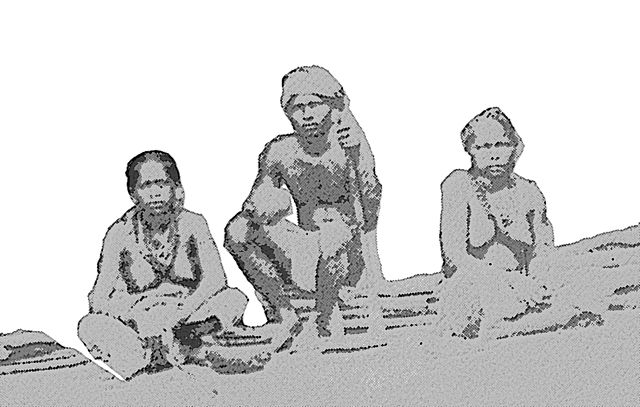
\includegraphics[width=0.7\textwidth,height=8cm]{Kulasthree_Chapter02_pic10.jpg}
\end{center}
\caption*{പുലയർ - കെ പി പത്മനാഭ മേനോൻ - വാള്യം 3, (1929), 1984}
\end{figure}

വരേണ്യസ്ത്രീകൾക്ക് ഇടയ്ക്കു ലഭിച്ചിരുന്ന വിനോദവേളകളും അവർക്കുണ്ടായിരുന്ന സുരക്ഷയും തീരെയില്ലാതെ, ഒരിക്കലും തീരാത്ത അദ്ധ്വാനത്തിൽ കഴിഞ്ഞ ജീവിതങ്ങളായിരുന്നു കീഴാള സ്ത്രീകളുടേത്. 20-ാം നൂറ്റാണ്ടിന്റെ ആരംഭത്തിൽ അവരുടെ അദ്ധ്വാനത്തെക്കുറിച്ച് ഒരു ലേഖകൻ/ലേഖിക എഴുതിയത് ഇങ്ങനെയാണ്:
\begin{quotation}
\noindent ഇനി നമുക്ക് വേലക്കാരെയും കർഷകരെയുംകുറിച്ച് ചിന്തിക്കാം. അവരുടെയിടയിൽ നിലം ഉഴുതിടുക, കിളയ്ക്കുക, വിറകുവെട്ടുക, തെങ്ങിൽ കയറുക മുതലായ ജോലികൾ പുരുഷന്മാർ ചെയ്യാറുണ്ട്. സ്ത്രീകൾ ചാമ്പൽ, ചാണകം, തോല് ഇതൊക്കെ തലച്ചുമടായി ചുമന്നുവന്ന് മണ്ണിൽ വളമായി ചേർത്തിളക്കുന്നു; നിലങ്ങളിൽ മുട്ടറ്റം ചേറിലും ചെളിയിലുംനിന്ന് ഞാറുപറിക്കുകയും നടുകയും ചെയ്യുന്നു; അവർതന്നെ കള പറിക്കുന്നു; വിളവു പാകമാകുമ്പോൾ കൊയ്യുന്നു; കറ്റ ചുമന്ന്, മെതിച്ച്, പാറ്റി, ചിക്കി, നെല്ലെടുക്കുന്നു; തൊണ്ട് വെള്ളത്തിലിട്ട്, തല്ലിപ്പിരിച്ച് കയറാക്കുന്നു; തെങ്ങോല മെടഞ്ഞ് പുരമേയാനുള്ളതുണ്ടാക്കുന്നു; പലതരം പായകളും തുണിയും നെയ്തെടുക്കുന്നു; തേങ്ങ ഉടച്ചുണക്കി കൊപ്രയാക്കി ആട്ടി എണ്ണയെടുക്കുന്നു; ഇതുകൂടാതെ പലതരത്തിലുള്ള ജോലികളിലും കൈവേലകളിലും ഏർപ്പെടുന്നു. നമ്മുടെ കൈവേലകൾ അധികവും പിന്തുടരുന്നത് സ്ത്രീകളാണെന്ന് സൂക്ഷ്മചിന്തയിൽ വ്യക്തമാകും. മാത്രമല്ല, ശൂദ്രരിൽ താഴെയുള്ള ജാതികളായ മാപ്പിള, തീയ്യ, കണക്ക, ചെറു, പുലയ, നായാടി മുതലായവയിൽ സ്ത്രീകളാണ് ശരീരത്തിനും മനസ്സിനും ആയാസമുള്ള ജോലികൾ, വളരെ കൂടുതൽ സമയം, ചെയ്യുന്നത്.\\
\\(കെ.പി.എം., 'സ്ത്രീകൾ അബലകളാണോ?', ലക്ഷ്മീഭായി 2 (8), 1907)
\end{quotation}

\paragraph{} പലതരം അദ്ധ്വാനമായിരുന്നു കീഴാളസ്ത്രീകളുടേത്. മേലാളന്മാർക്കുവേണ്ടി ഉത്പാദനപരമായ അദ്ധ്വാനം മാത്രമല്ല അവർ ചെയ്തിരുന്നത് - പാടത്തു പണിയെടുക്കുന്നതിനു പുറമെ മേലാളരുടെ വീടുകൾക്കു ചുറ്റുമുള്ള പല പണികളും അവർ ചെയ്തുവന്നു. മേലാളപുരുഷന്മാരെ ലൈംഗികമായി സന്തോഷിപ്പിക്കുന്നതിനും അവർ നിയോഗിക്കപ്പെട്ടു. കേരളത്തിലെ ജാതിവ്യവസ്ഥയുടെ പ്രത്യേകത 'തീണ്ടൽ' ആയിരുന്നുവെന്നകാര്യം പ്രസിദ്ധമാണല്ലോ. കീഴ്ജാതിക്കാരെ തൊട്ടുകൂടെന്നു മാത്രമല്ല, അവരെ സമീപത്തു കണ്ടാൽപോലും 'അശുദ്ധ'മാകുമെന്ന വിശ്വാസമാണ് 'തീണ്ടൽ'. പക്ഷേ, ഇക്കാര്യത്തിന് 'തീണ്ടലൊ'ന്നും ബാധകമായിരുന്നില്ല - അതു കുളിച്ചാൽ പോകുമെന്നായിരുന്നു വിശ്വാസം! കൃഷിയിടങ്ങളിൽനിന്ന് പണിശാലകളിലേക്ക് - ഫാക്ടറികളിലേക്ക് - കീഴാളർ 20-ാം നൂറ്റാണ്ടിൽ നീങ്ങിത്തുടങ്ങിയപ്പോൾ (കാണുക \ref{11.3}) ഈ കഠിനവ്യവസ്ഥ അവരെ പിന്തുടർന്നു. കശുവണ്ടിത്തൊഴിലാളികളായി മാറിയവരുമായി അന്നാ ലിന്റ്ബർഗ് (Anna Lindberg) നടത്തിയ അഭിമുഖസംഭാഷണങ്ങളിൽ ഇതു തെളിയുന്നുണ്ട് (കാർഷികരംഗത്ത് വളരെക്കാലം ഇതു തുടർന്നുവെന്നു സൂചിപ്പിക്കുന്ന പഠനങ്ങൾ വേറെയുണ്ട്).
\paragraph{}തിരുവിതാംകൂർ പ്രദേശത്തുനിന്ന് മലബാർഭാഗത്തേക്ക് കൃഷിഭൂമിതേടിയുള്ള കർഷകരുടെ കുടിയേറ്റം ഇരുപതാംനൂറ്റാണ്ടിന്റെ പകുതിയോടെ ശക്തിപ്രാപിച്ചു തുടങ്ങിയിരുന്നു. അങ്ങനെ സ്ഥലംമാറി കാടുകൾ വെട്ടിത്തെളിക്കാൻ പുറപ്പെട്ട കുടുംബങ്ങളിലെ സ്ത്രീകളുടെ അതികഠിനമായ അദ്ധ്വാനത്തെക്കുറിച്ച് നിരവധി കഥകൾ - സാഹിത്യരൂപത്തിലും അല്ലാതെയും - ഇന്നു നാം കേൾക്കുന്നുണ്ട്. മലമ്പനിയെയും കാട്ടുമൃഗങ്ങളെയും ഭയന്ന്, രാപ്പകൽ കൃഷിഭൂമിയിൽ അദ്ധ്വാനിച്ചുകൊണ്ട് സ്വന്തം കുടുംബങ്ങളുടെ നില ഭദ്രമാക്കാൻ അവർ തീവ്രമായി പരിശ്രമിച്ചു. പുരുഷൻ ചെയ്ത എല്ലാ ജോലികളും ചെയ്തു, കൊടും തണുപ്പിലും. തുല്യമായി പണിയെടുക്കുകയെന്നത് പിടിച്ചുനിൽക്കാനുള്ള ഏകമാർഗ്ഗമായിരുന്നതുകൊണ്ട് 'സ്ത്രീക്ക് വീട്ടുപണി, പുരുഷന് കൂലിപ്പണി' മുതലായ ഇന്നത്തെ സാമാന്യബോധമൊന്നും അവിടെ അന്നു ചെലവാകുകയില്ലായിരുന്നു! ഒരേ പണി ചെയ്തതുപോലെ സ്ത്രീപുരുഷന്മാർ ഒന്നിച്ചിരുന്നു പുകവലിക്കുകയും മദ്യം കഴിക്കുകയും ചെയ്യുന്നത് ആദ്യകാലങ്ങളിലൊന്നും വലിയ ഞെട്ടലുളവാക്കിയിരുന്നില്ലെന്നു പഴമക്കാർ പറഞ്ഞുകേട്ടിട്ടുണ്ട്.

\paragraph{}ഫാക്ടറികളിലെ കീഴാളരായ സ്ത്രീത്തൊഴിലാളികളിൽനിന്ന് ലൈംഗികമായ വിധേയത്വം പ്രതീക്ഷിച്ചിരുന്നുവെന്ന് മുതിർന്ന സ്ത്രീകൾ ചരിത്രഗവേഷകയായ അന്നയോട് പറഞ്ഞു. മുതലാളിമാർ നടത്തിയ സൽക്കാരങ്ങളിലുംമറ്റും 'സഹകരിക്കാൻ' ചില സ്ത്രീകളോട് ആവശ്യപ്പെട്ടിരുന്നത്രെ; ഇതുകൂടാതെ മുതലാളിമാരുടെ റൗഡിസംഘങ്ങൾ സ്ത്രീകളെ ഉപദ്രവിക്കുന്നത് തെറ്റായി അംഗീകരിച്ചിരുന്നില്ല. 1918ൽ ജനിച്ച ദേവകി എന്ന ഈഴവസമുദായാംഗമായ തൊഴിലാളിസ്ത്രീയുടെ ഓർമ്മയിൽനിന്ന്:
\begin{quotation}
\noindent ....[ഇത്തരം ഉപദ്രവം] എത്ര സാധാരണയായിരുന്നെന്ന് പറയാൻ എനിക്കു കഴിയില്ല. പക്ഷേ, ഞാനത് പലതവണ കണ്ടിട്ടുണ്ട്. പഴയ ദിവാൻഭരണകാലത്തായിരുന്നു ഇത് [1930കളിലും 40കളിലും]. വളരെ സുന്ദരിയായ ഒരു പുലയ പെൺകുട്ടിയെ ഞാനോർക്കുന്നു. അവർ കുറച്ചു വൈകല്യമുള്ള ഒരു സഹോദരിയോടൊപ്പം ഈ ഗ്രാമത്തിൽ ഒരു കൂരയിലായിരുന്നു താമസിച്ചിരുന്നത്. നല്ല പെൺപിള്ളാരെ അന്വേഷിച്ച് മൂപ്പൻ [തൊഴിലാളികളെ കണ്ടെത്തി ഫാക്ടറിയിലെത്തിക്കുന്നയാൾ] ഇങ്ങോട്ടുവരുമ്പോൾ അവൾ എപ്പോഴും താഴേക്കുനോക്കി നിൽക്കും; പക്ഷേ, അവർക്ക് അവളെത്തന്നെ വേണം. അവള് കഷ്ടപ്പെടുന്നുവെന്ന് ഞങ്ങൾക്കൊക്കെ കാണാമായിരുന്നു, പക്ഷേ, അവൾ ഒന്നും മിണ്ടിയിരുന്നില്ല. ഒരു പാവം പെണ്ണ് എന്തുചെയ്യാനാ? ഒരുദിവസം അവളും സഹോദരിയും അവിടുന്നങ്ങു പോയി - ആർക്കും അറിയില്ല, എങ്ങോട്ടേക്കെന്ന്. എന്നാൽ അവൾ എന്തുകൊണ്ട് പോയെന്ന് ഞങ്ങൾക്കറിയാമായിരുന്നു.\\
\\(Anna Lindberg, Experience and Identity, പുറം 144)
\end{quotation}
\paragraph{}എന്നാൽ കുടുംബസംവിധാനത്തിനുള്ളിൽ കീഴാളസ്ത്രീകൾ കൂടുതൽ സ്വാതന്ത്ര്യം അനുഭവിച്ചിരുന്നുവെന്നും വ്യക്തമാണ്. വിവാഹമോചനം എളുപ്പമായിരുന്നു; വിധവാവിവാഹവും പുനർവിവാഹവും സാധാരണ സംഭവങ്ങളായിരുന്നു. ജനിച്ചിടത്തുനിന്ന് മറ്റൊരിടത്തേക്ക് മാറിപ്പാർക്കാൻ അവർക്കു സ്വാതന്ത്ര്യമുണ്ടായിരുന്നു. കുടുംബത്തിനുള്ളിൽ തീരുമാനങ്ങൾ അവരുടെ പങ്കാളിത്തത്തോടുകൂടിയാണ് എടുത്തിരുന്നത്. ഭർത്താവിനോട് തുറന്നുതന്നെ വിയോജിക്കുന്ന രീതി വളരെ സാധാരണമായിരുന്നു; അത് 'അനുസരണക്കേടാ'യി വ്യാഖ്യാനിച്ചിരുന്നില്ല. 1960ൽ പ്രസിദ്ധീകരിച്ച തന്റെ പുസ്തകത്തിൽ സാമൂഹ്യശാസ്ത്രജ്ഞനായ കെ.സി. അലക്സാണ്ടർ ഇതു ശ്രദ്ധിക്കുന്നുണ്ട്. ഒരേ പാത്രത്തിൽനിന്ന് ഭക്ഷണം കഴിക്കുക, ഭർത്താവു കയറിവരുമ്പോൾ ഭാര്യ എഴുന്നേൽക്കാതിരിക്കുക ഇതൊക്കെ 1950കളിലും കീഴാളകുടുംബങ്ങളിൽ സാധാരണയായിരുന്നത്രെ. അതേസമയം ജാതിവ്യവസ്ഥയുടെ കാർക്കശ്യം അനുഭവിച്ചിരുന്ന ഈഴവർ സാമ്പത്തികപുരോഗതി നേടുകയും ലിംഗബന്ധങ്ങളിൽ (നവീകരിക്കപ്പെട്ട) ബ്രാഹ്മണമൂല്യങ്ങളെ അനുകരിക്കുകയും ചെയ്തുകഴിഞ്ഞിരുന്നു. കീഴാളരുടെയിടയിൽ, പക്ഷേ, കുടുംബത്തിനുള്ളിൽ സ്ത്രീകൾ വളരെക്കാലം, വലിയൊരളവുവരെ, തുല്യതയനുഭവിച്ചു. കർഷകത്തൊഴിലാളിസംഘടനകളിലും, ഫാക്ടറികളിലെ സംഘടനകളിലും കീഴാളസ്ത്രീകൾ ഭർത്താവിന്റെ സമ്മതം നോക്കാതെതന്നെ അംഗങ്ങളായിരുന്നുവെന്ന് ഗവേഷകൻ നിരീക്ഷിച്ചിട്ടുണ്ട്. എന്നാൽ കശുവണ്ടിമേഖലയിലെ നായർ-ഈഴവസമുദായാംഗങ്ങളായ സ്ത്രീത്തൊഴിലാളികൾ ഭർത്താവിന്റെ സമ്മതത്തിനായി പലപ്പോഴും കാത്തിരുന്നുവെന്ന് ലിന്റ്ബർഗിന്റെ പഠനം സൂചിപ്പിക്കുന്നു. കീഴാളസ്ത്രീകൾ തൊഴിലാളികളായിരുന്നു; കൂലി അവർക്കു പണമായി കൈയിൽ കിട്ടിയിരുന്നു. പൊതുസ്ഥലങ്ങളിൽ പോകാൻ അവർക്കു വിലക്കില്ലായിരുന്നു. ഇന്ന് പുരുഷന്മാരുടേതുമാത്രമായിത്തീർന്നിരിക്കുന്ന പല ഇടങ്ങളും രീതികളും അന്ന് സ്ത്രീകളും പങ്കുവച്ചിരുന്നുവെന്ന് ലിന്റ്ബർഗിനോടു സംസാരിച്ച മുതിർന്ന സ്ത്രീകളിൽ പലരും പറയുന്നു. 1919ൽ ജനിച്ച പുലയസമുദായാംഗമായ കോത ഇതേക്കുറിച്ചു പറഞ്ഞത്:
\begin{quotation}
\noindent അതേ, ഈയടുത്തകാലത്ത് പെണ്ണുങ്ങൾ 'പെണ്ണുങ്ങളാ'യിരിക്കണമെന്നാണ്... ഞങ്ങളുടെ ചെറുപ്പത്തിൽ അങ്ങനെയായിരുന്നില്ല. ഞങ്ങൾ വെള്ളം കോരിക്കൊണ്ടുവന്നു, വിറകും ചാണകവും പെറുക്കി, ഇതൊക്കെക്കൂടാതെ വേറെയും ഒത്തിരി ജോലി ചെയ്തു.... (പക്ഷേ) ഞങ്ങളും ഇടയ്ക്കൊക്കെ ഒന്ന് ആഘോഷിച്ചിരുന്നു. അതായത്, കള്ളുകുടിക്കാൻ പോകുമ്പോൾ - ആണുങ്ങളുടെയത്രയില്ല, എങ്കിലും.... ഇന്ന് ഒറ്റ സ്ത്രീയും കള്ളുകുടിക്കാൻ പോവില്ല. അതൊക്കെ ആണുങ്ങളുടെ സ്ഥലമായി... പല ചെറുപ്പക്കാരികൾക്കും രാത്രിയായാൽ പുറത്തിറങ്ങാൻ പേടിയാണ്. ഒരുപാടു കുടിയന്മാരും അക്രമവുമൊക്കെയുണ്ട് - പണ്ടങ്ങനെയായിരുന്നില്ല. മുതലാളിയുടെ ഗുണ്ടകളെയാണ് ഞങ്ങൾ പേടിച്ചിരുന്നത്. മുതലാളിയുടെ സ്വകാര്യസൈന്യംപോലെയായിരുന്നു അവർ.\\
\\(Anna Lindberg, Experience and Identity, പുറം 263)
\end{quotation}
\section{തിരിഞ്ഞു ചിന്തിക്കുമ്പോൾ}
\paragraph{}വിവാഹം, ദായക്രമം എന്നിവയെമാത്രം പരിഗണിച്ചുകൊണ്ട് കേരളത്തെ 'പെണ്ണരശുനാട്' എന്നു വിളിച്ചതിൽ അർത്ഥമില്ലായിരുന്നുവെന്ന് വ്യക്തമാകുന്നു. മരുമക്കത്തായത്തിൽ സ്ത്രീകൾക്ക് അനുകൂലമായ ഘടകങ്ങൾ ഉണ്ടായിരുന്നുവെന്നത് നേരുതന്നെ; പക്ഷേ, ഈയൊരൊറ്റക്കാരണംകൊണ്ട് നാട്ടിൽ 'പെൺഭരണമാ'യിരുന്നുവെന്ന് തീർച്ചപ്പെടുത്താൻ കഴിയില്ല. മാത്രമല്ല, മരുമക്കത്തായം സ്ത്രീകൾക്കു നൽകിയിരുന്ന അവകാശങ്ങളും അധികാരങ്ങളും 19-ാം നൂറ്റാണ്ടുമുതൽ ക്ഷയിച്ചു [ 49 ] എന്നുവേണം പറയാൻ. വരേണ്യസ്ത്രീകൾക്ക് ഭാരിച്ച ഗാർഹിക ഉത്തരവാദിത്വങ്ങളുമുണ്ടായിരുന്നു. കീഴാളസ്ത്രീകളുടെ നിലകൂടി പരിഗണിച്ചാൽ 'സ്ത്രീസ്വാതന്ത്ര്യത്തെ പരമ്പരാഗതമായിത്തന്നെ പ്രാത്സാഹിപ്പിച്ചവർ' എന്ന ഖ്യാതിയൊന്നും നമുക്കവകാശപ്പെടാനില്ലെന്നും വ്യക്തം!
\paragraph{}എങ്കിലും കേരളത്തിന്റെ ഈ പേര് ഇന്നും നിലനിൽക്കുന്നുണ്ട്, പലയിടങ്ങളിലും. കേരളത്തിലെ സാമൂഹികവികസനത്തെക്കുറിച്ചുള്ള ചർച്ചകളിലും പലരും ഇതിനെക്കുറിച്ച് പരാമർശിക്കാറുണ്ട്. വിദ്യാഭ്യാസം, ആരോഗ്യം, ജനസംഖ്യാനിയന്ത്രണം മുതലായ മേഖലകളിൽ കേരളം ഉണ്ടാക്കിയ നേട്ടങ്ങളെക്കുറിച്ചു പറയുമ്പോൾ, പരമ്പരാഗത മരുമക്കത്തായം സ്ത്രീകൾക്കു നൽകിയ സ്വാതന്ത്ര്യം, പെൺകുഞ്ഞുങ്ങൾക്കു കല്പിച്ച വില, ഇവയെക്കുറിച്ച് പ്രത്യേകം പരാമർശങ്ങളുണ്ടാകാറുണ്ട്. ഒരളവുവരെ ഇതിൽ ശരിയുണ്ട് - ഉദാഹരണത്തിന്, മരുമക്കത്തായത്തിൽ സ്ത്രീകൾക്ക് പഠിപ്പ് പൂർണ്ണമായി നിഷേധിക്കപ്പെട്ടിരുന്നില്ല; പലപ്പോഴും സ്ത്രീകൾക്ക് നല്ല വിദ്യാഭ്യാസം നേടാൻ കഴിഞ്ഞിരുന്നു. വീടുകൾക്കുള്ളിൽ അടഞ്ഞുകിടന്നുകൊള്ളണമെന്ന നിബന്ധന അവർക്കു ബാധകമായിരുന്നില്ല. അതുകൊണ്ട് 19-ാം നൂറ്റാണ്ടിൽ തിരുവിതാംകൂർ-കൊച്ചി രാജ്യങ്ങൾ പെൺപള്ളിക്കൂടങ്ങൾ ആരംഭിച്ചപ്പോൾ തങ്ങളുടെ പെൺമക്കളെ അവിടേക്കയയ്ക്കാൻ മരുമക്കത്തായക്കാർ മടിച്ചില്ല. പക്ഷേ, ഇങ്ങനെ ഗുണകരമായ ഒരു വ്യവസ്ഥയെ നാട്ടിൽനിന്ന് അടിച്ചോടിക്കാതെ ഈ നാട് ഗുണംപിടിക്കില്ലെന്ന പല്ലവിയാണ് സാമൂഹ്യപരിഷ്ക്കർത്താക്കൾ 19-ാം നൂറ്റാണ്ടിലും അതിനുശേഷവും പാടിയത്! അതായത് നാമിന്ന് സാമൂഹികവികസനമെന്ന് വിളിക്കുന്ന നേട്ടങ്ങൾ രൂപപ്പെട്ടകാലത്തുതന്നെയാണ് മരുമക്കത്തായം ഈ നാട്ടിൽനിന്നു നിഷ്ക്കാസനം ചെയ്യപ്പെട്ടതും. ഇക്കാലത്തെ സാമൂഹ്യമാറ്റങ്ങൾകൊണ്ട് നാടിനു ഗുണമുണ്ടായിട്ടില്ലെന്നല്ല. പക്ഷേ, സ്ത്രീകളുടെ സ്വന്തം താൽപര്യങ്ങൾക്ക്, സ്വയംപര്യാപ്തതയ്ക്ക് ഉതകുന്ന എന്തൊക്കെ സാഹചര്യങ്ങൾ ഇവയിലൂടെ ഉണ്ടായി എന്നുകൂടി പരിശോധിക്കേണ്ടതാണ്.
\section{കൂടുതല്‍ ആലോചനയ്ക്ക്}
\paragraph{}നിലവിലുള്ള പ്രബലധാരണകളെ പൊളിച്ചെഴുതിക്കൊണ്ടാണ് സ്ത്രീചരിത്രം ചരിത്രപഠനരംഗത്ത് സ്വന്തമായൊരിടം ഉറപ്പിച്ചത്. ആധുനിക കേരളചരിത്രത്തിന്റെ പശ്ചാത്തലത്തിലും ഈ സാദ്ധ്യത നിലനിൽക്കുന്നുണ്ട്. കേരളത്തിലെ സ്ത്രീകളുടെ ചരിത്രാനുഭവങ്ങളെക്കുറിച്ച് സാധാരണക്കാർക്കിടയിലും പണ്ഡിതവൃത്തങ്ങളിലും പ്രബലമായി നിലനിൽക്കുന്ന ഒരു ധാരണയാണ് ഈ അദ്ധ്യായത്തിൽ പുനഃപരിശോധിക്കപ്പെട്ടത്. സ്ത്രീകളെ 'പാടിപ്പുകഴ്ത്തല'ല്ല സ്ത്രീചരിത്രത്തിന്റെ ഏകധർമ്മമെന്നും ഈ അദ്ധ്യായത്തിൽ കൈക്കൊണ്ട സമീപനം വ്യക്തമാക്കുന്നു. സ്ത്രീകളുടെ അംഗീകരിക്കപ്പെട്ടിട്ടില്ലാത്ത ചരിത്രാനുഭവങ്ങളെ, സംഭാവനകളെ, വെളിച്ചത്തു കൊണ്ടുവരുക എന്നത് അതിന്റെ പല ധർമ്മങ്ങളിലൊന്നുമാത്രമാണ്. സ്ത്രീകളെ 'പുകഴ്ത്താനുള്ള' എല്ലാ ശ്രമങ്ങളും അവർക്ക് അനുകൂലമായിക്കൊള്ളണമെന്നില്ലെന്ന് ഈ അദ്ധ്യായം വാദിക്കാൻ ശ്രമിക്കുന്നു. പലപ്പോഴും സ്ത്രീകൾക്ക് അനുകൂലമല്ലാത്ത സ്ഥാപനങ്ങളെയും സമ്പ്രദായങ്ങളെയും നമ്മുടെ ശ്രദ്ധയിൽനിന്ന് അകറ്റിനിർത്താനാണ് ഈ പുകഴ്ത്തൽ ഉപകരിക്കുന്നത്. 'സ്ത്രീകൾ' എന്നാൽ മരുമക്കത്തായവ്യവസ്ഥയ്ക്കുകീഴിൽ കഴിഞ്ഞ സ്ത്രീകൾ മാത്രമല്ല എന്നുകൂടി കണക്കിലെടുക്കുമ്പോൾ മേൽപ്പറഞ്ഞ 'പുകഴ്ത്തൽ' എളുപ്പമാവില്ലെന്നു വ്യക്തമാണ്! 
\begin{figure}[h]
\begin{center}
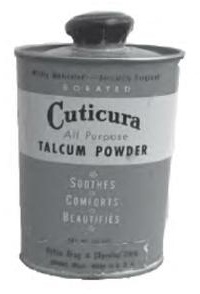
\includegraphics[width=0.5\textwidth,height=7cm]{Kulasthree_Chapter02_pic12.jpg}
\end{center}
\end{figure}


\section{കേരളത്തിന്റെ ചരിത്രകാരികൾ: മീരാ വേലായുധൻ}
\begin{figure}[h]
\begin{center}
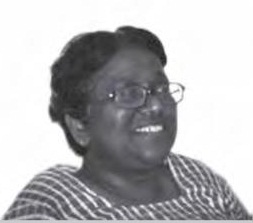
\includegraphics[width=0.5\textwidth,height=5cm]{Kulasthree_Chapter02_pic13.jpg}
\end{center}
%\caption*{}
\end{figure}
[ന്യൂഡൽഹിയിലെ ജാമിയ മില്ലിയ ഇസ്ലാമിയ സർവ്വകലാശാലയിൽ ഡോക്ടറൽ ഗവേഷണംനടത്തിയ മീരാ വേലായുധൻ ആധുനിക മലയാളിസ്ത്രീകളുടെ ചരിത്രത്തെക്കുറിച്ച് ആദ്യകാലത്ത് ഗവേഷണംനടത്തിയവരിലൊരാളാണ്. മലബാറിലെ രാഷ്ട്രീയ ഉണർച്ചയുടെ കാലത്ത് സ്ത്രീകളുടെ രാഷ്ട്രീയപങ്കാളിത്തത്തെക്കുറിച്ചും സാമുദായിക-രാഷ്ട്രീയപ്രസ്ഥാനങ്ങളിൽ അവരുടെ നിലയെക്കുറിച്ചും വിലപ്പെട്ട ഉൾക്കാഴ്ചയും വിവരങ്ങളും നൽകുന്ന ലേഖനങ്ങൾ അവർ പ്രസിദ്ധീകരിച്ചിട്ടുണ്ട്. ഇടതുപക്ഷത്തെ ആദ്യകാല സ്ത്രീപ്രവർത്തകരുമായി അവർ നടത്തിയ അഭിമുഖങ്ങൾ വളരെ വിലപ്പെട്ട സ്രോതസ്സാണ്.]

\paragraph{}

നീതിബോധത്തിന് പല ഉറവുകളാണുള്ളത് - ചരിത്രം; പിറന്ന, വളർന്ന, പരിചയിച്ച, സ്ഥലങ്ങൾ; സ്വത്വങ്ങൾ. എന്റെ നീതിബോധം മാതാപിതാക്കൾ പകർന്നുതന്നതാണ്. എന്റെ അമ്മയായ ദാക്ഷായണി വേലായുധൻ കൊച്ചി മുളവുകാട് ദ്വീപിലെ ഒരു മരുമക്കത്തായ പുലയത്തറവാട്ടിലാണ് ജനിച്ചത്. കളരിപ്പയറ്റും നാടകവും മറ്റു "നാടൻകല'കളും ഈ തറവാട്ടംഗങ്ങൾക്ക് പൈതൃകമായി ലഭിച്ചിരുന്നു. (ഒരിക്കൽ അവർ കടലിൽ ഒരു വള്ളത്തിൽ നാടകം നടത്തിയ കഥ പറഞ്ഞുകേട്ടിട്ടുണ്ട് - കടൽ ഉന്നതജാതിക്കാരുടെയും പണക്കാരുടെയും കുത്തകയല്ലായിരുന്നല്ലോ.) സ്ത്രീകൾ കൃഷിപ്പണി ചെയ്തിരുന്നു; മത്സ്യം ഉണക്കിയിരുന്നു. ഒരുപാടുകാര്യങ്ങളിൽ അവർ മുൻഗാമികളുമായിരുന്നു. എന്റെ അമ്മയും മറ്റൊരു കൂടപ്പിറപ്പുമൊഴിച്ച് മറ്റു കുഞ്ഞുങ്ങളെയെല്ലാംകൂട്ടി ക്രിസ്തുമതം സ്വീകരിച്ചയാളായിരുന്നു എന്റെ മുത്തശ്ശി. ഇളയസന്താനങ്ങൾക്ക് കൊച്ചി മഹാരാജാവു നൽകിയ സൗജന്യവിദ്യാഭ്യാസത്തിന്റെ ഗുണംകിട്ടണമെന്ന് അവർ ആഗ്രഹിച്ചിരുന്നു. മുളവക്കാട്ടു പള്ളിക്കൂടത്തിൽ മേൽമുണ്ടിട്ട ആദ്യത്തെ കീഴാളസ്ത്രീയായിരുന്നിരിക്കണം എന്റെ അമ്മ; കൊച്ചീരാജ്യത്തിലും ഇന്ത്യയിലും ആദ്യമായി ബിരുദവിദ്യാഭ്യാസം പൂർത്തിയാക്കിയ ദലിത് സ്ത്രീയായിരുന്നു അവർ. ക്ലാസിൽ എല്ലായ്പ്പോഴും ഒന്നാമതായിരുന്ന ബാലിക. പിന്നീട് സ്കൂൾ അദ്ധ്യാപികയായിത്തീർന്നപ്പോൾ, അവർ പൊതുവഴിയിലൂടെത്തന്നെ നടക്കുമെന്നുറച്ചു; മേൽജാതിക്കാർ അപ്പോൾ വയലിലൂടെ നടക്കാൻ നിർബന്ധിതരായി. സ്കൂളിൽ അദ്ധ്യാപകർ പുസ്തകങ്ങൾ തന്റെനേരെ വലിച്ചെറിയാൻ ദാക്ഷായണി അനുവദിച്ചിരുന്നില്ല; മര്യാദയ്ക്ക് കയ്യിൽക്കൊടുക്കാത്ത പുസ്തകങ്ങൾ അവർ സ്വീകരിച്ചിരുന്നില്ല. എന്നോട് അവരെപ്പോഴും പറഞ്ഞിരുന്നു, നേരേയിരിക്കൂ, തലയുയർത്തിയിരിക്കൂ, നമ്മുടെ കൂട്ടർക്ക് ഇതുവരെ തലതാഴ്ത്തിനടക്കാനായിരുന്നു വിധി. നാട്ടുരാജ്യപ്രസ്ഥാനങ്ങളിൽ അവർ ക്രമേണ സജീവപങ്കാളിയായി; ആജീവനാന്തം ഗാന്ധിയൻ ജീവിതരീതിയുടെ വക്താവായി. 1930കളുടെ മദ്ധ്യത്തിൽ ഉദ്യോഗം വേണ്ടെന്നുവച്ചുകൊണ്ട് അവർ കൊച്ചി നിയമസഭാകൗൺസിൽ അംഗമായി. പിൽക്കാലത്ത് അവർ ഇന്ത്യൻ ഭരണഘടനാനിർമ്മാണസഭയിലും ആദ്യത്തെ കേന്ദ്രനിയമസഭയിലും അംഗമായി. ബാബാ സാഹേബ് അംബേദ്കറുടെ ഉറച്ച അനുയായി അറിയപ്പെട്ടു. വാർധയിലെ ഗാന്ധി ആശ്രമത്തിൽവച്ചാണ് അവർ എന്റെ പിതാവായ രാമൻ വേലായുധനെ വിവാഹംചെയ്തത് - കസ്തൂർബയുടെയും ഗാന്ധിജിയുടെയും സാന്നിദ്ധ്യത്തിൽ. അതൊരു "പ്രണയവിവാഹ'മായിരുന്നു. 1970കളിൽ [ 52 ] ഡൽഹിയിലെ തൂപ്പുവേലയെടുക്കുന്ന സ്ത്രീകൾക്കിടയിൽ അവർ പണിയെടുത്തിരുന്നു; അഭ്യസ്തവിദ്യരായ ദലിത്‌സ്ത്രീകളുടെ ദേശീയ കൂട്ടായ്മയിൽ അംഗമായിരുന്നു. മരണത്തിന് അൽപ്പകാലംമുമ്പ് അവർ ഈ കൂട്ടായ്മയ്ക്കൊപ്പം (1970കളുടെ ഒടുക്കം) ദലിത്‌സ്ത്രീകളുടെ ദേശീയസമ്മേളനം ഡൽഹിയിൽ നടത്തി. ഞാൻ കൂടെപ്പോയിരുന്നു - അമ്മ ഇതിനായി വീടുവീടാന്തരം കയറിയിറങ്ങി ദലിത്‌ഭവനങ്ങളിൽനിന്ന് ധനശേഖരണം നടത്തിയപ്പോൾ. ഒടുവിൽ 'മഹിളാജാഗൃതീ പരിഷത്ത്' എന്ന പേരിൽ ഒരു അഖിലേന്ത്യ ദലിത്‌സംഘടയ്ക്ക് അവർ ജന്മംകൊടുത്തു. ഈ പ്രവർത്തനകാലംമുഴുവൻ അവർ എൽ.ഐ.സിയിൽ ഇൻഫർമേഷൻ ഉദ്യോഗസ്ഥയായി ജോലിനോക്കിയിരുന്നു. മിക്ക സ്ത്രീകളെയുംപോലെ, കുടുംബം പുലർത്തിയിരുന്നു. ഞാൻ 1990കളുടെ മദ്ധ്യത്തിൽ രൂപീകൃതമായ ദലിത്‌സ്ത്രീ ദേശീയ ഫെഡറേഷന്റെ ഭാഗമായിത്തീർന്നത് യാദൃശ്ചികമായല്ല; ആ ബന്ധം പണ്ടേയുണ്ടായിരുന്നു.
\paragraph{}

എന്റെ അച്ഛൻ പഴയ ജന്മിത്ത തിരുവിതാംകൂറിലെ ഉഴവൂർ പ്രദേശത്തുള്ള ഒരു പരവകുടുംബത്തിൽനിന്നാണ്. അദ്ദേഹത്തിന്റെ അച്ഛൻ ആയുർവ്വേദ വൈദ്യനായിരുന്നതുകൊണ്ട് അവരുടെ ജന്മി മക്കളെ പള്ളിക്കൂടത്തിലയയ്ക്കാനനുവദിച്ചു. അദ്ദേഹത്തിന്റെ സഹോദരന്മാർ ജനസമ്മതിയാർജ്ജിച്ച കർഷകനേതാക്കളായിരുന്നു, കേരളത്തിന്റെ കാർഷികചരിത്രത്തിൽ അവർ അദൃശ്യരാണെങ്കിലും. ഗാന്ധിജിയാണ് എന്റെ അച്ഛനെ കണ്ടെടുത്തത്, കോളജിൽ നടന്ന ഒരു പ്രതിഷേധസമരത്തിനിടയിൽനിന്ന്. ബോംബെയിൽ ടാറ്റാ ഇൻസ്റ്റിറ്റ്യൂട്ടിൽനിന്ന് സാമൂഹ്യശാസ്ത്രം പഠിച്ചിറങ്ങിയ ആദ്യ വിദ്യാർത്ഥികളിലൊരാളായിരുന്നു അദ്ദേഹം. സോഷ്യലിസ്റ്റ് രാഷ്ട്രീയത്തോടടുത്തശേഷം രണ്ടു ലോക്സഭാ തെരഞ്ഞെടുപ്പുകളിൽ അദ്ദേഹം വിജയിച്ചു - അന്ന് സംവരണമണ്ഡലമല്ലായിരുന്ന കൊല്ലത്തുനിന്ന്. രണ്ടാമത്തെ തവണ ഇടതുസ്വതന്ത്രനായാണ് മത്സരിച്ചത്. ഡൽഹിയിൽ പലവിധത്തിലുള്ള ഇടതുരാഷ്ട്രീയപ്രവർത്തനങ്ങളിലും ട്രേഡ്‌യൂണിയൻ പ്രവർത്തനങ്ങളിലും പങ്കാളിയായിരുന്നു. അദ്ദേഹം നടത്തിയിരുന്ന നിരവധി യാത്രകളിലൂടെ കുട്ടികളായ ഞങ്ങൾക്ക് ലോകത്തിന്റെ പല ഭാഗങ്ങളിലും നടക്കുന്ന കാര്യങ്ങളെക്കുറിച്ച് ബോധമുണ്ടായി. അവസാനനാളുകളിൽ ബുദ്ധമതത്തോട് അദ്ദേഹം പ്രതിപത്തികാട്ടിയിരുന്നു.
\paragraph{}

വീട്ടിൽ ഞങ്ങൾ മലയാളം സംസാരിച്ചിരുന്നെങ്കിലും വടക്കേയിന്ത്യയിൽ ജനിച്ചുവളർന്നതുകൊണ്ട് ഹിന്ദിയാണ് മാതൃഭാഷയായി എനിക്ക് അനുഭവപ്പെട്ടിരുന്നത്. എങ്കിലും പലയിടങ്ങളിലും വേരുകളുണ്ടെന്ന തോന്നൽ എപ്പോഴും എനിക്കുണ്ടായിരുന്നു. ബിരുദാനന്തരപഠനത്തിനുശേഷം ഞാൻ നടത്തിയ ഗവേഷണമധികവും കേരളത്തിലായിരുന്നു. കേരളത്തിനു പുറത്തു ജീവിക്കേണ്ടിവന്നതിൽ എന്റെ അമ്മ അനുഭവിച്ച നഷ്ടബോധത്തെ ഏതോ വിധത്തിൽ പരിഹരിക്കാനുള്ള എന്റെ ശ്രമമായിരുന്നിരിക്കാം, ഒരുപക്ഷേ, ഇത്!
\paragraph{}

അഞ്ചുമക്കളിൽ ഏകമകളായിരുന്നു ഞാൻ എന്നതുകൊണ്ട് അച്ഛനമ്മമാരുടെയും ആങ്ങളമാരുടെയും പ്രത്യേക പരിഗണന എനിക്കുണ്ടായിരുന്നു. തുടർച്ചയുള്ള വിദ്യാഭ്യാസം എനിക്കു ലഭിക്കണമെന്ന് അവർക്ക് നിർബന്ധമായിരുന്നു. പലപ്പോഴും ഫീസിനുംമറ്റും ഞങ്ങൾ ബുദ്ധിമുട്ടിയിരുന്നു. പക്ഷേ, വിദ്യാലയകാലത്തുതന്നെ എന്റെ ജീവിതം ഞാൻതന്നെ കെട്ടിപ്പടുക്കുമെന്ന തീരുമാനത്തിൽ ഞാൻ എത്തിക്കഴിഞ്ഞിരുന്നു. ഒരു 'രാഷ്ട്രീയവ്യക്തി'യാണ് ഞാനെന്ന് തികഞ്ഞ അഭിമാനബോധത്തോടെ പ്രഖ്യാപിക്കാൻ എനിക്ക് അച്ഛന്റെ പ്രരണയുമുണ്ടായിരുന്നു. 1980കളുടെ സവിശേഷസാഹചര്യങ്ങളിലാണ് എന്റെ ബുദ്ധിപരവും രാഷ്ട്രീയവുമായ ബോധം രൂപമെടുത്തത്. പ്രത്യേകിച്ച്, ഞാൻ സ്ത്രീപ്രസ്ഥാനത്തിന്റെ ഭാഗമായിത്തീർന്നത്. എല്ലായ്പ്പോഴും ഞാൻ തെരഞ്ഞെടുപ്പുകൾ നടത്തിയത് നീതിബോധത്തോടുകൂടിയാണ് - എന്റെ അച്ഛനമ്മമാരെപ്പോലെ തന്നെ.
